% !TeX spellcheck = it_IT
\title{Tecniche di Protezione del Software}
\author{Massimo Perego}
\date{}

\documentclass[11pt]{article}
\usepackage{graphicx} 
\usepackage{amsmath}
\usepackage{amssymb}
\usepackage{amsfonts}
\usepackage[autostyle, english = american]{csquotes}
\usepackage[parfill]{parskip}
\MakeOuterQuote{"}

\usepackage{xcolor}
\definecolor{bg}{rgb}{0.95,0.95,0.95}
\definecolor{g}{rgb}{0,0.5,0.1}
\usepackage{minted}
\setminted[c]{linenos, bgcolor=bg}
\setminted[java]{bgcolor=bg}
\usepackage[hidelinks]{hyperref}
\usepackage{tikz}
\usepackage{enumitem}
\usepackage{array}
\usepackage{booktabs}
\usepackage{adjustbox}

%\includeonly{chapters/sme}
%\includeonly{chapters/tme}
%\includeonly{chapters/mts}
%\includeonly{chapters/rop}
%\includeonly{chapters/cfi}
%\includeonly{chapters/vulnerabilities}
%\includeonly{chapters/fuzzing}
%\includeonly{chapters/side}

\renewcommand{\contentsname}{Indice}

\begin{document}
	\maketitle
	\tableofcontents
	\newpage	
	
	% !TeX spellcheck = it_IT
%Insomma: 
%4 lezioni sugli attacchi low level
%4 lezioni sulle difese low level
%5 lezioni su fuzzing, side channel, symbolic execution, analisi di programmi
%TL;DR: attacco, difesa, analisi
\section{Spatial Memory Errors}
%Slide 0 Buffer Overflow - Intro

Ci concentriamo su linguaggi low level (e.g., C), i quali tendono a crashare in caso di errori (come buffer overflow), ma un attaccante può \textbf{sfruttare le vulnerabilità} per ottenere informazioni (e.g., Heartbleed, bug SSL che permetteva di leggere tutta la memoria del programma, che su SSL insomma, peso), corrompere memoria, fino ad arbitrary code execution (la macchina comincia ad eseguire altro, diventa una "weird machine"), ecc.\\
Il crash (ovvero \texttt{segfault}), se analizzato può portare ad un attacco, anche se non tutti i casi sono exploitabili (molti sì).\\

Questo tipo di bug hanno una lunga storia e sono tuttora presenti, e lo saranno finché C e C++ saranno usati. Inoltre è utile studiare l'evoluzione del bug stesso, assieme alle difese create per contrastarlo. Alcune caratteristiche di un attacco/difesa possono risultare presenti anche in altri attacchi.\\

Inoltre, solitamente, l'attacco è molto più semplice della difesa. Per l'attacco mi basta un punto, per la difesa devo essere sicuro di aver coperto tutti i possibili punti di attacco, senza degradare troppo le performance.\\

I sistemi C e C++ sono ancora molto presenti e spesso sono parte di sistemi critici come: 
\begin{itemize}
	\item OS, Kernel e relative utilities
	\item Server che richiedono alte prestazioni (Apache httpd, nginx, MySQL, redis)
	\item Sistemi embedded (risorse limitate, le performance sono importanti)
\end{itemize}

La prima versione di buffer overflow funzionante è del 1988: Morris Worm, per poi dare inizio ad una catena di exploit che permettono la compromissione della macchina stessa (a diversi livelli), in qualsiasi caso con un impatto significativo.\\

\newpage

%Slide 1 Buffer Overflow - Memory Layout
\subsection{Memory Layout}
Dobbiamo sapere come un programma viene caricato in memoria, in quali zone e di conseguenza cos'è lo stack e quali sono gli effetti delle chiamate a funzione. Parleremo del modello Linux \texttt{x64}, anche se il concetto dell'attacco è universale l'implementazione può cambiare in base a dettagli tecnici (architectural dependent).\\

\textbf{Ogni processo} ha un proprio \textbf{layout di memoria}, con indirizzi che vanno da \texttt{0x00000000} a \texttt{0xffffffff} (per 32 bit, con 64 sarebbero troppo lunghi da scrivere), quindi 4GB di indirizzamento totali.\\

Linux divide:
\begin{itemize}
	\item 1GB per il sistema operativo, dall'alto
	\item 3GB per le applicazioni
\end{itemize}
Di conseguenza il primo indirizzo valido per il programma è \texttt{0xbfffffff}, sopra c'è il kernel.\\

Il \textbf{loader carica in memoria} un \textbf{processo} quando questo viene chiamato, occupando la page table ed allestendo la memoria per l'uso del programma. \\

\newpage

Il loader divide la memoria (tra quella adibita al programma, i 3GB di prima) in sezioni:
\begin{itemize}
	\item \textbf{Text} per memorizzare il codice del programma
	\item Zone per dati inizializzati (\textbf{Data}) e non (Block Started by Symbol \textbf{BSS})
\end{itemize}
Queste sono \textbf{conosciute a compile time}, mentre
\begin{itemize}
	\item \textbf{Stack}
	\item \textbf{Heap}
\end{itemize}
Sono \textbf{dinamiche} e permettono la gestione del programma.
\begin{center}
	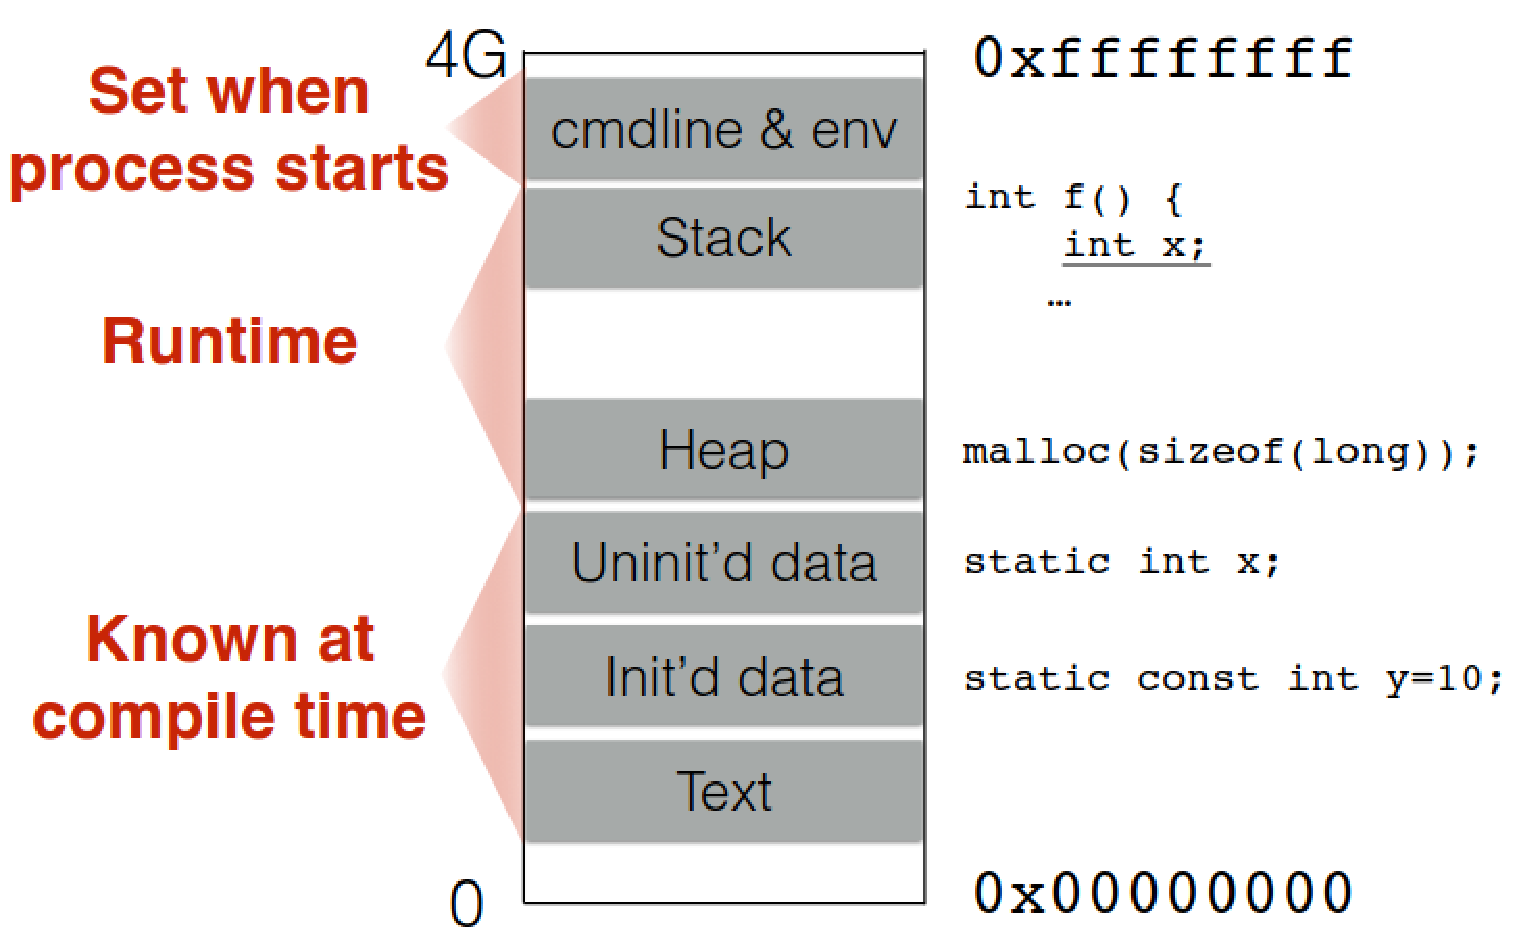
\includegraphics[width=0.85\linewidth]{img/sme/memory_all1}
\end{center}

Stack e Heap quindi sono zone dinamiche che \textbf{crescono in direzioni opposte} (stack verso il basso).\\
Nell'heap ci sono le allocazioni dinamiche effettuate dal programmatore stesso (\texttt{malloc} e simili), mentre lo \textbf{stack} viene \textbf{gestito dal compilatore} per memorizzare cose come le chiamate a funzione. \\

\newpage

\subsubsection{Stack}
All'interno dello stack viene gestita l'esecuzione del programma. Gli \textbf{indirizzi dello stack crescono verso il basso}, partendo da \texttt{0xbfffffff} e scendono. Questo rende possibile l'attacco di buffer overflow stack based, nel modo attualmente esistente.\\

Man mano che viene allocata memoria, lo stack alloca spazio dall'alto verso il basso. \texttt{Push} decrementa il valore dell'indirizzo, \texttt{Pop} lo aumenta.\\

\paragraph{Stack Pointer:} Su architetture Intel, si tratta del \textbf{registro} che tiene conto dell'\textbf{indirizzo a cui è arrivato lo stack}, il valore dello spazio allocato più in basso (ultimo valore allocato, da dove posso ricominciare ad allocare).\\

Il compilatore utilizza lo stack quando vengono chiamate le funzioni, \textbf{nel momento in cui avviene una chiamata a funzione}:
\begin{itemize}
	\item viene effettuata la \texttt{push} (istruzione macchina) dei parametri della funzione sullo stack
	\item l'istruzione macchina \texttt{call} viene chiamata, portando l'esecuzione all'indirizzo di memoria del codice della funzione
	\item la \texttt{call} effettua anche la \texttt{push} sullo stack dell'indirizzo di ritorno di una funzione, ovvero da dove proseguire l'esecuzione al termine della funzione 
\end{itemize} 
%Viene effettuata la push e poi la call? Check

Dopo queste istruzioni comincia l'esecuzione della funzione. All'\textbf{interno dello stack} vengono \textbf{memorizzate le variabili locali}, quindi viene effettuata una \texttt{push} di queste variabili all'interno dello stack.\\

\newpage

Al termine dell'esecuzione ci sarà un'istruzione \texttt{ret} che fa tornare l'\textbf{esecuzione all'indirizzo puntato dal return address} memorizzato in precedenza sullo stack (anche senza \texttt{return} esplicito, serve a continuare l'esecuzione del programma dopo la funzione).\\

La funzione di \texttt{ret}: 
\begin{itemize}
	\item libera la zona dedicata alle variabili locali, \texttt{pop} di tutte le variabili memorizzate sullo stack
	\item carica nell'instruction pointer (o program counter, registro che tiene traccia dell'istruzione da eseguire) il valore del return address (indirizzo della prossima istruzione che deve eseguire il processore)
\end{itemize}
Bisogna deallocare anche i parametri allocati sullo stack ma chi lo effettua dipende dalla calling convention del compilatore, quindi può farlo il chiamato o il chiamante (i.e., il pop di quei valori verrà effettuato prima o dopo il \texttt{ret}).\\

In ordine, dall'alto verso il basso, all'interno dello stack saranno presenti: 
\begin{itemize}
	\item Parametri 
	\item Return address
	\item Variabili locali
\end{itemize}

\newpage

\subsection{Stack-based Overflow}

Esempio di bug: 
\begin{minted}{c}
void f (par){
	char buf[10];
	strcpy(buf, par);
}
\end{minted}

La funzione \textbf{non controlla dimensioni di sorgente e destinazione}, quindi cosa succede se l'\textbf{elemento da copiare è più grande} della \textbf{memoria} che gli è stata \textbf{allocata} (ovvero la dimensione del buffer destinazione)?\\

Lo \textbf{stack} sarà \textbf{composto da}:
\begin{itemize}
	\item parametri della funzione, \texttt{par} in questo caso
	\item return address
	\item variabili locali, qui solo il buffer destinazione
\end{itemize} 

Se la dimensione del buffer da copiare è maggiore del buffer allocato il programma \textbf{andrà a sovrascrivere i valori precedenti nello stack} (lo stack alloca dall'alto verso il basso, ma gli indirizzi del buffer vanno dal basso verso l'alto, l'indice 1 è più in basso dell'indice 8, per mantenere coerente l'aritmetica con i puntori, I guess). \\

Il valore sopra il buffer nello stack è il return address, che porterà a tornare ad un indirizzo casuale se sovrascritto, portando ad un \texttt{segfault}.\\

Non c'è un controllo che limiti la scrittura alla dimensione del buffer, portando a sovrascrivere altre parti dello stack.\\

\newpage

\subsubsection{Code Injection}
Come possiamo sfruttare questa situazione? Tramite buffer overflow posso avere il controllo sul return address; control flow hijacking.\\

Per arrivare ad \textbf{eseguire codice arbitrario} devo
\begin{itemize}
	\item definire il codice
	\item iniettarlo in memoria
	\item cambiare il valore del return address in modo che punti a quella zona di memoria
\end{itemize}

\paragraph{Definire il codice:} Il processore legge solamente stringhe di byte che corrispondono alle istruzioni da eseguire. Noi dobbiamo costruire un bytestream a partire da del codice sorgente che vogliamo eseguire. Un bytestream che chiama \texttt{/bin/bash} diventa uno shellcode.\\
Dobbiamo forgiare un bytestream adatto alle nostre esigenze, manualmente prendendolo da del codice eseguito o tramite tool appositi (più facile solitamente).

\paragraph{Injection Vector:} Per metterlo in memoria, il posto ideale sarebbe il \textbf{buffer} che abbiamo \textbf{già a disposizione}. L'\textbf{input} viene \textbf{copiato nel buffer}, il quale è sullo stack. Quindi inserendo il bytestream all'interno dell'input posso inserirlo in memoria all'interno del buffer.\\

Dobbiamo \textbf{costruire un input} che fa partire l'esecuzione del codice voluto (chiamato injection vector). Sarà quindi composto dal \textbf{bytestream del codice} (e.g., shellcode) e dal \textbf{valore che sovrascriverà il return address}, ovvero l'indirizzo del buffer (come trovarlo?). \\
Nell'esempio sopra ci saranno 10 byte per lo shellcode (dimensione allocata per il buffer) e 4 byte per il return address (considerando architetture a 32 bit).\\
In questo modo, quando il programma torna dalla funzione, porrà nel program counter l'indirizzo del buffer, contenente il bytestream forgiato da noi. La sequenza di istruzioni posta nel buffer sarà quindi interpretata come codice. Abbiamo dirottato il control flow, portando all'esecuzione di codice arbitrario.\\

\paragraph{Spatial memory error:} Stiamo "mischiando" dati dell'utente e control channel (comandi di controllo), problematica comune a più vulnerabilità e possibili ambiti. Sovrascriviamo nello spazio dei caratteri di controllo. L'esecuzione di codice arbitrario avviene al ritorno della funzione vulnerabile.\\

Adesso ci sono protezioni che bloccano esecuzione di codice all'interno dello stack, non è una zona di memoria che dovrebbe contenere codice (anche se ci sono anche casi particolari) e l'esecuzione di codice presente in zone di memoria simili è bloccata.\\

%End L1

\newpage

\subsection{Heap}

\subsubsection{Heap vs Stack}
Lo \textbf{stack} è principalmente gestito dal compilatore per allocazioni \textbf{statiche} della memoria, conosciute a compile time. Inoltre tutti i metadati utili al programma sono memorizzati sullo stack. Un esempio di metadato è il return address per il ritorno di una funzione. \\

Questo è solitamente nascosto al programmatore, se la dimensione dei dati non è nota a priori viene usato l'\textbf{heap}, una memoria comandata (allocazione e liberazione) dal programmatore tramite funzioni di libreria. Generalmente più lenta ed a \textbf{gestione manuale}.  Solitamente usato per oggetti, structs ed in generale elementi più grandi.\\

Lo stack cresce dell'alto verso il basso (indirizzi), mentre l'heap cresce dal basso verso l'alto. Una \texttt{push} sullo stack sposta il \texttt{rsp} verso il basso (e, di conseguenza, la \texttt{pop} verso l'alto). In caso di un utilizzo troppo elevato di memoria si possono "incontrare" le due zone (hai finito la memoria).\\

La vulnerabilità già vista sullo stack nasce dal "mischiare" dati inseriti dall'utente con metadati che permettono di alterare il flusso di controllo del programma.\\

le due funzioni principali per gestire la memoria nell'heap sono: 
\begin{itemize}
	\item \texttt{malloc(size)}: restituisce un puntatore ad una zona di memoria con dimensione \texttt{size}
	\item \texttt{free(ptr)}: dato un puntatore, libera la zona di memoria associata
\end{itemize}

%\subsubsection{Heap overflow}
Anche nell'heap sono presenti metadati, e di conseguenza la possibilità di sovrascriverli, portando a possibili vulnerabilità.\\

\paragraph{Allocatori:} Definiti nelle librerie di sistema, per gestire le zone di memoria allocate servono comunque dei metadati. L'allocatore gestisce i propri dati all'interno dell'heap stesso (problema di canale).

\newpage

\subsubsection{Heap Chunk} 

\paragraph{Heap Chunk:} Struttura dati per la memoria nell'heap. Struttura:
\begin{minted}{c}
struct malloc_chunk {
	INTERNAL_SIZE_T 	prev_size; 
	INTERNAL_SIZE_T 	size; 
	
	struct malloc_chunk* 	fd;
	struct malloc_chunk* 	bk;
	
	struct malloc_chunk* 	fd_nextsize;
	struct malloc_chunk* 	bk_nextsize;
	};
\end{minted}
I ordine, i parametri sono:
\begin{itemize}
	\item \texttt{prev\_size}: dimensione della zona di memoria precedente, usato solo se il chunk è libero
	\item \texttt{size}: dimensione della zona di memoria occupata da questo chunk, overhead compreso
	\item \texttt{fd}, \texttt{bk}: puntatori alle zone di memoria precedenti e successive nella lista di chunk liberi (e di conseguenza presenti solo se il blocco è libero)
	\item \texttt{fd\_nextsize}, \texttt{bk\_nextsize}: puntatori alle dimensioni degli elementi adiacenti nella lista di chunk liberi (usati solo se il chunk è libero)
\end{itemize}
\begin{center}
	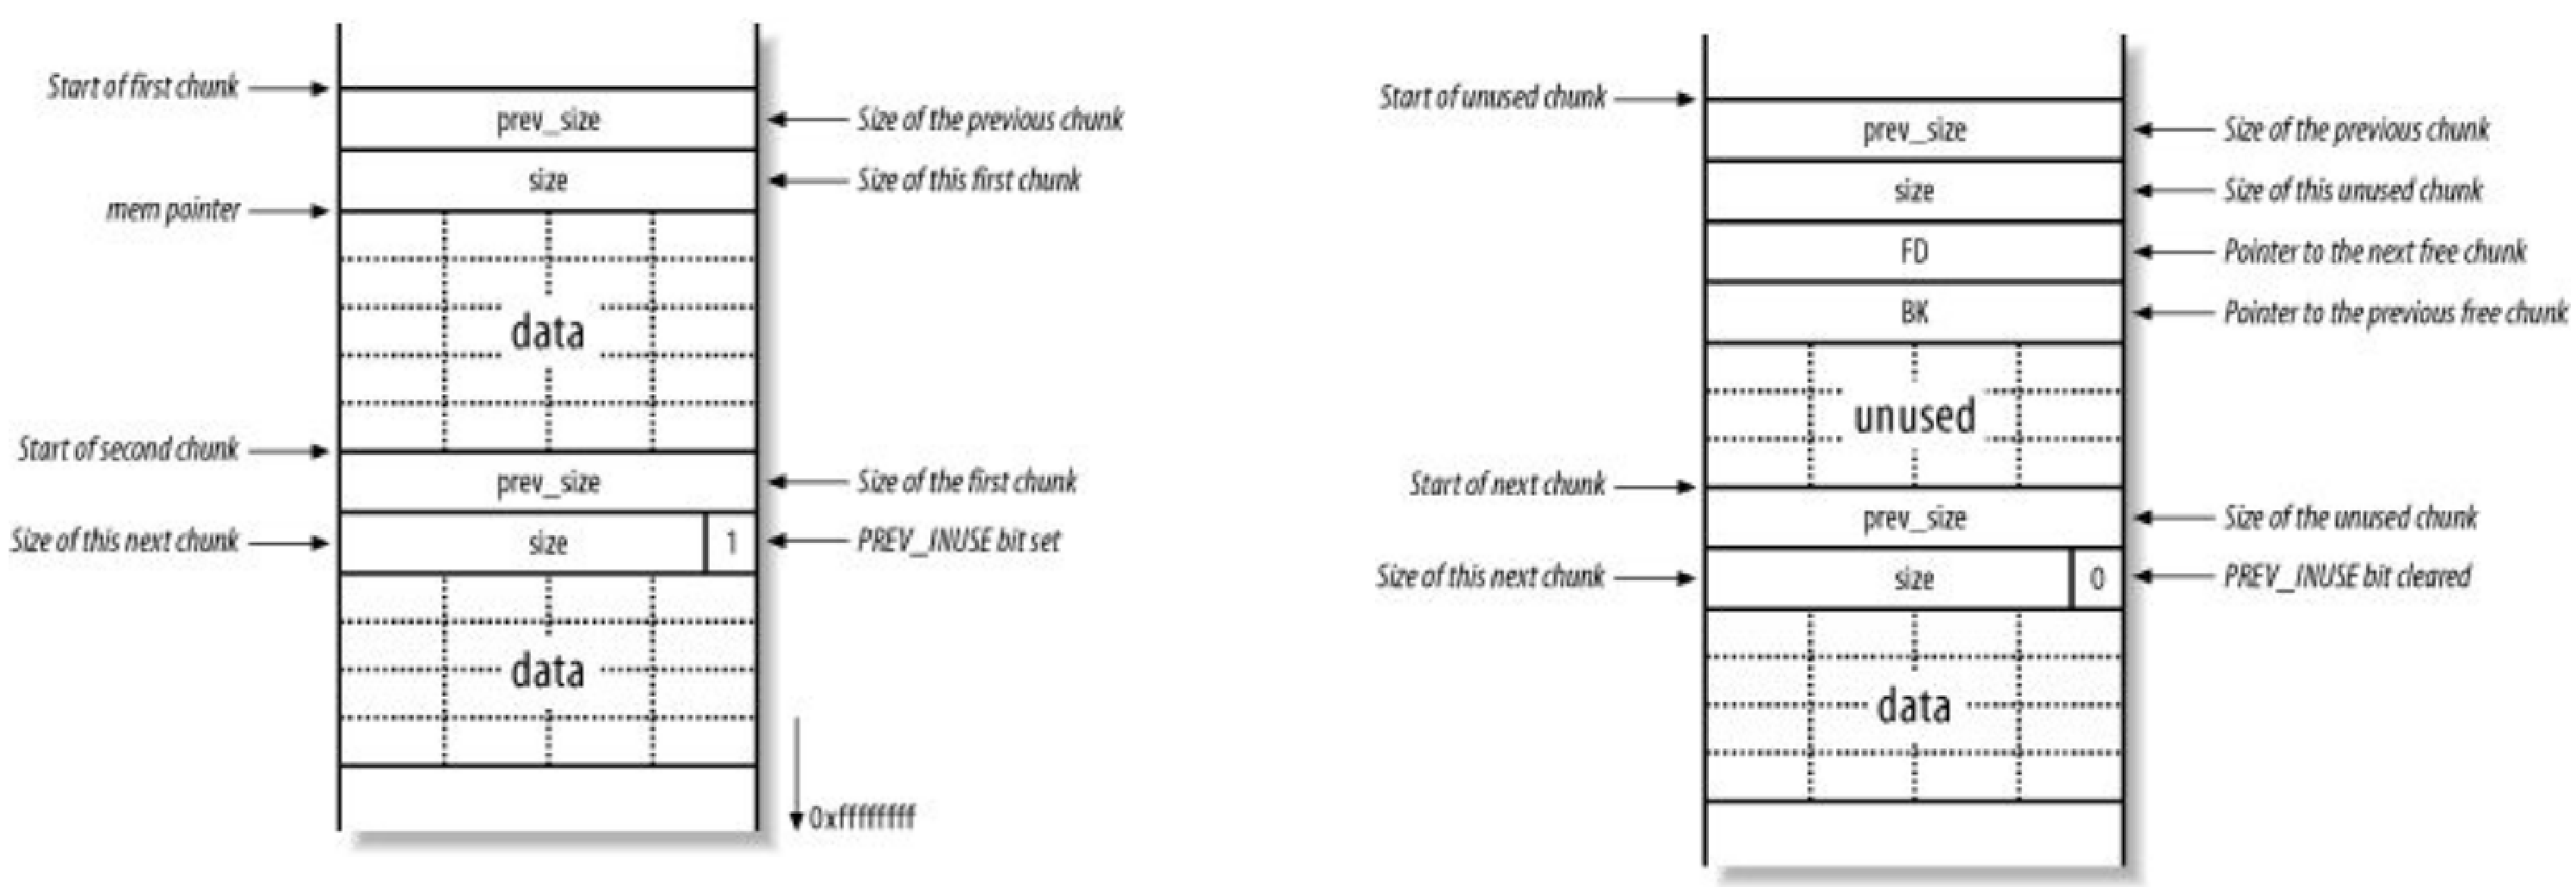
\includegraphics[width=\linewidth]{img/sme/heapchunk}
\end{center}
I chunk occupati contengono solo \texttt{size} e i dati. Il puntatore di ritorno ottenuto tramite \texttt{malloc} punta all'inizio della zona contenente i dati. \\

\newpage

\subsubsection{Allocare e deallocare memoria}

\paragraph{Allocazione:} All'inizio dell'esecuzione si ha un top chunk, che rappresenta tutta la grandezza dell'heap. Si ha un puntatore al top chunk chiamato \texttt{av\_top}; inizialmente questo puntatore coincide con la base della memoria. In seguito ad una \texttt{malloc}, viene allocata la zona di memoria richiesta, restituendo i relativi puntatori, e di conseguenza  \texttt{av\_top} viene spostato "sopra" al blocco allocato, deve puntare sempre alla zona di memoria "rimanente"; il top chunk decresce in seguito all'allocazione.\\

\paragraph{Deallocazione:} Oltre allo spazio libero del top chunk sono presenti delle liste di free chunk, una per ogni dimensione di chunk liberi (se posso occupare la memoria esatta lo faccio, serve a ridurre la frammentazione). Quando viene richiesta un'allocazione, prima cerca se c'è una zona di memoria "grande giusta" (o poco più, se mi servono 256 byte cerco nella lista di blocchi liberi da 256 byte), se non c'è una zona adatta nelle liste di chunk liberi allora prende la memoria dal top chunk.\\

Nel caso in cui due chunk adiacenti diventino liberi, vengono collassati in uno solo e lo inserisce nella lista rilevante.\\

\vfill

\begin{minipage}{0.43\textwidth}
	\textbf{Allocazione:}
	\begin{itemize}
		\item Richiesta di memoria (\texttt{malloc})
		\item Ricerca di un blocco libero (prima dalle liste, eventualmente si usa il top chunk)
		\item Aggiornamento della struttura di gestione (metadati)
		\item Restituzione del puntatore
	\end{itemize}
\end{minipage}
\hfill
\begin{minipage}{0.43\textwidth}
	\textbf{Deallocazione:}
	\begin{itemize}
		\item Richiesta di rilascio (\texttt{free})
		\item Il blocco viene marcato come libero 
		\item Coalescenza di blocchi adiacenti (se presenti, si fondono blocchi liberi adiacenti in uno solo)
		\item Aggiornamento della struttura di gestione
	\end{itemize}
\end{minipage}

\newpage

\subsection{Heap Overflow}

\subsubsection{Unlink}
Quando viene effettuata una allocazione bisogna aggiornare i puntatori, il nodo occupato va "sganciato" dalla lista (doppiamente concatenata) di blocchi liberi, e di conseguenza i puntatori del blocco successivo e precedente vanno aggiornati (sai come si rimuove un elemento da una lista dai). La procedura è
\begin{minted}{c}
void unlink(malloc_chunk *P, malloc_chunk *BK, 
	malloc_chunk *FD) {
		FD = P->fd;
		BK = P->bk;
		FD->bk = BK;
		BK->fd = FD;
}
\end{minted}
Dove: 
\begin{itemize}
	\item \texttt{P} nodo da eliminare
	\item \texttt{BK} nodo precedente
	\item \texttt{FD} nodo successivo 
\end{itemize}
"Stacco" il nodo da eliminare facendo puntare il puntatore \texttt{bk} del nodo successivo al nodo precedente e viceversa.\\

\newpage

\subsubsection{Exploit "Naive"}
Se non è presente nessun controllo durante le scritture, una write troppo grande può andare a sovrascrivere i chunk (liberi o occupati) superiori, metadati compresi.\\

Nello specifico, posso sovrascrivere il \texttt{FD->bk} e \texttt{P->bk}, rispettivamente con l'indirizzo di un return address e un indirizzo di un buffer (injection vector).\\
\begin{minted}{c}
	FD->bk = return address address;
	FD = P->fd;
	BK = P->bk = address of the buffer;
	FD->bk = BK;
\end{minted}

Partendo da un heap con dei chunk liberi e la relativa lista, facendo overflow in un chunk occupato sottostante si può sovrascrivere il puntatore \texttt{bk} di due chunk vuoti con indirizzi determinati dall'attaccante (rispettivamente, un blocco con inizio di un buffer con codice malevolo, il blocco dopo con l'indirizzo del return address di una funzione).\\

Quando il programma andrà ad allocare il primo dei blocchi con i valori sovrascritti dovrà rimuoverlo dalla lista di blocchi liberi, quindi eseguire la procedura di unlink: il \texttt{bk} del blocco "sganciato" punta al buffer contenente qualcosa (e.g., shellcode, inizio di un buffer controllato dall'attaccante, in qualsiasi modo), mentre il \texttt{bk} blocco successivo punta al return address di una funzione, il quale verrà sovrascritto con l'indirizzo del buffer (procedura di unlink), portando il programma ad eseguire il codice all'interno del buffer una volta che il programma dovrà seguire il return address sovrascritto.\\

Questo exploit è stato patchato controllando che \texttt{FD} e \texttt{BK} puntino effettivamente l'uno all'altro, non si può più sparare allo stack.\\

%up to s11
% Missing House of Force attack

\newpage

\subsubsection{House of Force}

Dopo la patch per la correzione dell'unlink sono nate nuove tecniche per sfruttare l'heap overflow, le principali si chiamano:
\begin{itemize}
	\item The House of Prime
	\item The House of Mind
	\item \textbf{The House of Force}
	\item The House of Lore
	\item The House of Spirit
	\item The House of Chaos
\end{itemize}

Verrà mostrata solo la House of Force, spiegazioni ed esempi per le altre possono essere trovate \href{https://github.com/shellphish/how2heap}{\texttt{a questo indirizzo}}. Ognuna di queste sfrutta diverse funzionalità dell'allocatore per attuare un attacco.\\

Tutte le tecniche citate hanno delle \textbf{condizioni per poter essere utilizzate}, la sola presenza della vulnerabilità non vuol dire che possa essere sfruttata.\\

Il \textbf{fuzzing} è il processo di trovare vulnerabilità nel programma, cercando crash del programma. Dopo aver trovato la vulnerabilità (i.e., il crash) bisogna analizzare se nel punto del programma che causa il crash ci sono le condizioni per un attacco vero e proprio, c'è da capire su che possibile vulnerabilità bisogna concentrarsi.\\

Un possibile ambito di ricerca sono gli AEG Automatic Exploit Generation: software per costruire in automatico attacchi a partire da possibili vulnerabilità (crash).\\

\newpage

Esempio di programma vulnerabile ad House of Force:
\begin{minted}{c}
char *buf1, *buf2, *buf3;

buf1 = malloc(256);
strcpy(buf1, argv[1]);

buf2 = malloc(strtoul(argv[2], NULL, 16));
buf3 = malloc(256);
strcpy(buf3, argv[3]);

free(buf3);
free(buf2);
free(buf1);
\end{minted}

Condizioni necessarie per questo exploit:
\begin{itemize}
	\item avere una prima malloc su un numero arbitrario di byte (fisso, non importante, \texttt{buf1} nell'esempio)
	\item avere una \texttt{strcpy()} sul buffer precedente (\texttt{buf1})
	\item avere un'altra \texttt{malloc} comandata dall'attaccante, i.e., la cui dimensione è definita in modo dinamico tramite input, in qualche modo (\texttt{buf2})
	\item avere un'altra \texttt{malloc} non comandata dall'attaccante, in cui l'attaccante può scrivere (anche in modo controllato, basta poter scrivere)
\end{itemize}
Al termine del programma ci saranno le free.\\

\newpage

Cosa succede sull'heap quando queste tre condizioni sono soddisfatte?
%Disegno
% Heap, rettangolo 
% Prima situazione: top chunk su tutto l'heap, con freccia per av\_top al termine
% Mostra l'allocazione del primo buffer, dal basso verso l'alto, mostra puntatore
% Mostra che la strcpy permette di sovrascrivere i metadati del top chunk

\begin{center}
	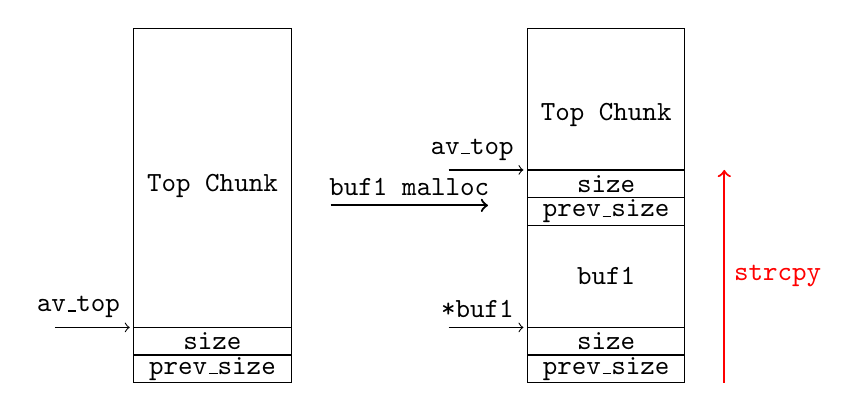
\begin{tikzpicture}[scale=0.5]
		% Draw the main rectangle
		\draw (0,0) rectangle (4,9);
		
		% Draw the divisions
		\draw (0,0.7) -- (4,0.7); % Bottom small section
		\draw (0,1.4) -- (4,1.4); % Middle small section
		
		% Labels
		\node at (2,5) {\texttt{Top Chunk}}; % Large section label
		\node at (2,1.05) {\texttt{size}}; % Middle small section label
		\node at (2,0.35) {\texttt{prev\_size}}; % Bottom small section label
		
		\draw[->] (-2,1.4) -- (-0.1,1.4);
		\node[above left] at (-0.1,1.4) {\texttt{av\_top}};
		
		\draw[thick, ->] (5,4.5) -- (9,4.5);
		\node[above] at (7,4.5) {\texttt{buf1 malloc}};
		
		% Draw the main rectangle
		\draw (10,0) rectangle (14,9);
		
		% Draw the divisions
		\draw (10,0.7) -- (14,0.7); % Bottom small section
		\draw (10,1.4) -- (14,1.4); % Middle small section
		
		\draw (10,4) -- (14,4); 
		\node at (12,2.7) {\texttt{buf1}};
		
		\node at (12,1.05) {\texttt{size}}; % Middle small section label
		\node at (12,0.35) {\texttt{prev\_size}}; % Bottom small section label
		
		\draw (10,4.7) -- (14,4.7); % Bottom small section
		\draw (10,5.4) -- (14,5.4); % Middle small section
		
		\node at (12,5.05) {\texttt{size}}; % Middle small section label
		\node at (12,4.35) {\texttt{prev\_size}}; % Bottom small section label
		
		\node at (12,6.8) {\texttt{Top Chunk}};
		
		\draw[->] (8,1.4) -- (9.9,1.4);
		\node[above left] at (9.9,1.4) {\texttt{*buf1}};
		
		\draw[->] (8,5.4) -- (9.9,5.4);
		\node[above left] at (9.9,5.4) {\texttt{av\_top}};
		
		\draw[red, thick, ->] (15,0) -- (15,5.4);
		\node[red, right] at (15,2.7) {\texttt{strcpy}};
	\end{tikzpicture}
\end{center}

Quindi possiamo arrivare a sovrascrivere la \texttt{size} del top chunk, permettendo di dire al programma quanto spazio libero rimane all'interno. Questa è il primo problema: metadato size del top chunk modificabile dall'attaccante. A questo punto posso "incrementare" la memoria dell'heap (dimensione di \texttt{size}) fino a \textbf{tutta la memoria del processo indirizzabile}, la \texttt{size} è determinata unicamente in modo software. Posso andare ad indirizzare nell'intera memoria del processo.\\

Una volta "allargato tutto", l'attaccante può andare in un punto arbitrario della memoria da sovrascrivere. L'heap adesso include stack, .text ed in generale tutta la memoria. Posso sovrascrivere una zona di memoria arbitraria con un qualsiasi valore. Ad esempio, sovrascrivendo un \texttt{return address} sullo stack.\\

Abbiamo ingannato l'allocatore per \textbf{includere lo stack nello spazio indirizzabile dall'heap}, permettendoci di sovrascrivere una zona di memoria arbitraria.\\

La seconda \texttt{malloc} ha un'ampiezza comandata dall'attaccante, il che ci permette di \textbf{raggiungere la base dello stack}, dove c'è il \texttt{return address} che si vuole sovrascrivere (questa è una dimensione variabile, $\Delta$ tra posizione \texttt{dell'av\_top} e posizione del \texttt{return address}, da calcolare).\\

\newpage

Dopo una \texttt{malloc} di dimensione $\Delta$, l'\texttt{av\_top} sarà nello stack, la terza allocazione di dimensione $n$ (fissa), partirà dall'\texttt{av\_top} (in questo momento stiamo presupponendo non ci siano liste libere, altrimenti bisogna stare un po' più attenti) e quando comincio a scrivere in quest'ultimo buffer (ultima \texttt{strcpy}, comandata dall'attaccante) starò sovrascrivendo il \texttt{return address}, magari con un indirizzo di una zona di memoria il cui contenuto è controllato dall'attaccante (anche nell'heap, generalmente la zona dati non è eseguibile, ma ci sono dei casi in cui potrebbe esserlo).\\

\vfill 

\paragraph{TL;DR:} Inganniamo l'allocatore nel pensare che il top chunk sia più grande di quanto non sia realmente, tramite overflow, per poi andare a sovrascrivere una zona di memoria arbitraria in una scrittura successiva.\\

%Esempi e utilizzo sul link
	
	% !TeX spellcheck = it_IT
\section{Temporal Memory Errors}

Le vulnerabilità viste fin'ora si basavano su un "problema" nello spazio relativo alla memoria (overflow di \textit{qualcosa}), invece, le vulnerabilità basate sulla rottura della temporal memory si focalizzano su una sequenza di esecuzione in ordine temporale. 

La \textbf{vulnerabilità si presenta in un certo istante di esecuzione} del programma, ovvero in uno stato specifico in cui il programma si trova.

Sono difficili da individuare con una revisione manuale del codice dato che serve conoscere la sequenza esatta di allocazione e deallocazione durante l'esecuzione del programma, difficilmente individuabile su codice complesso.

\subsection{Use After Free UAF}

Una \textbf{Use-After-Free} accade quando si \textbf{usa un puntatore che è stato precedentemente liberato} (dereferenziazione di un puntatore che punta a una zona di memoria liberata, dangling pointer).

Esempio: 
\begin{minted}{c}
char *a, *b; int i;

a = malloc(16);
b = a + 5;
free(a);

b[2] = 'c';   /* use after free */
b = retptr();
*b = 'c';     /* use after free */
\end{minted}

Conoscere l'insieme di puntatori che puntano a un oggetto, senza una struttura dati come il garbage collector, non è un problema semplice (\textbf{aliasing} problem). 

Un analizzatore statico solitamente non riesce a trovare tutti gli aliasing, inoltre possono esserci puntatori definiti dinamicamente sulla base dell'oggetto.

Per avere una UAF bisogna individuare: 
\begin{itemize}
	\item una allocazione
	
    \item una deallocazione
	
    \item una dereferenziazione su un qualcosa di deallocato
\end{itemize}

Dopo averla individuata bisogna sfruttarla, tramite la funzione dell'allocatore che effettua la ricerca nelle liste di blocchi liberi un elemento della esatta grandezza richiesta, i.e., se la grandezza è giusta, riallocherà la zona allocata in precedenza.

Se c'è la possibilità, dopo la deallocazione, di eseguire una \texttt{malloc()} di dimensione e valori controllati, il dangling pointer precedente punterà ai dati scritti dall'attaccante (quelli che sono rimasti nella zona deallocata e successivamente re-allocata). 

La UAF è la vulnerabilità più frequente \textit{in natura}, più difficile da scovare e spesso permette di arrivare a esecuzione di codice arbitrario.

% End l4

	% !TeX spellcheck = it_IT

\section{Memory Safety and Type Safety}

Tutti gli errori descritti nelle sezioni precedenti nascono da un \textbf{utilizzo errato della memoria}, nei linguaggi che lo permettono. 

Utilizzare \textbf{linguaggi memory safe} permetterebbe di evitare le problematiche descritte precedentemente, ma il degrado delle performance potrebbe non essere accettabile per alcuni casi d'uso.

Memory safety e type safety sono due proprietà intrinseche ad alcuni linguaggi di programmazione che permettono di bloccare la possibilità di effettuare gli attacchi descritti in precedenza.

Le \textbf{difese} possono essere a \textbf{livello} di: 
\begin{itemize}
	\item \textbf{compilatore}: come le canary, usate per rilevare una eventuale sovrascrittura del return address

	\item \textbf{sistema operativo}: come l'Address Space Layout Randomization ASLR, che impedisce di sapere le posizioni esatte dei valori in memoria

	\item \textbf{architetturale}: componenti hardware che permettono di bloccare gli attacchi
\end{itemize}

Per contrastare ASLR sono nati gli attacchi Return Oriented Programming ROP (vedi \ref{sec:rop}), e per contrastare questi esiste la Control Flow Integrity CFI (vedi \ref{sec:cfi}, controllo sulle transizioni del programma, se va "fuori dagli schemi", ad esempio modificando il return address, la transizione è bloccata).

\subsection{Memory Safety}

Sicurezza della memoria, si tratta di una proprietà fondamentale di alcuni linguaggi (detti memory safe). 

Un programma scritto in un linguaggio memory safe:
\begin{itemize}
	\item Permette di creare puntatori solo attraverso alcuni mezzi standard; si vogliono intercettare i punti di creazione dei puntatori

	\item Permette di usare puntatori solo per accedere a memoria che "appartiene" a quel puntatore; un puntatore che appartiene a una zona di memoria deve accedere effettivamente a quella zona di memoria
\end{itemize}

Combina le idee di temporal safety (accedere solo a memoria attualmente allocata/valida) e spatial safety (accedere solo a memoria valida).

\subsubsection{Spatial safety}

Permette di far valere la proprietà di \textbf{sicurezza spaziale della memoria}, ovvero controllare che un puntatore non vada a puntare oltre una zona di memoria stabilita.

\paragraph{Fat Pointers:} Un puntatore non è più "solo un puntatore", ma diventa una tripla $(p,b,e)$ dove:
\label{par:fat-pointers}
\begin{itemize}
	\item $p$ è il puntatore effettivo
    
	\item $b$ è la base della zona di memoria a cui può accedere
	
    \item $e$ è l'estensione/limite della zona a cui può accedere
\end{itemize}

L'accesso è permesso se e solo se 
$$b \leq p \leq e - \text{\texttt{sizeof(typeof(} $p$ \text{\texttt{))}}} $$

Ogni puntatore ha un tipo, quindi "quanto si può spostare" è determinato anche dalla dimensione del tipo puntato (se è su \texttt{int} di 4 byte non posso puntare al penultimo byte, andrei fuori per gli ultimi 3). 

L'aritmetica sui puntatori modifica solo $p$, senza toccare $b$ ed $e$; $p$ si sposta, gli altri due rimangono lì per stabilire i limiti. Deve sempre valere la disuguaglianza.

I Fat Pointers sono \textbf{puntatori che hanno dati aggiuntivi}, come la tripla descritta in precedenza; metadati aggiunti ai puntatori. 

Effettuare il \textbf{controllo a ogni accesso} degrada le performance (soprattutto quando non è l'unico controllo da effettuare, questo è solo per la spatial safety). Il controllo è oneroso e necessita memoria aggiuntiva per i metadati legati a ogni puntatore.

Il compilatore di un linguaggio memory safe deve istanziare memoria aggiuntiva, \textit{per ogni puntatore}, e aggiungere il codice per i controlli, \textit{a ogni accesso}.

\vfill

\paragraph{Implementazione naive:}
\begin{minted}{c}
typedef struct {
    int *ptr;
    size_t e;
} fint_ptr;

fint_ptr make_fint(size_t n) {
    fint_ptr f;
    f.ptr = malloc(n * sizeof(int));
    f.e = n;
    return f;
}

bool get_fint(fint_ptr f, size_t i, int *out) {
    if (i < 0 || i > f.e)
        return false;
    *out = *f.ptr + i;
    return true;
}

void free_fint(fint_ptr *f) {
    free(f->ptr);
    f->ptr = NULL;
    f->e = 0;
}
\end{minted}

\paragraph{Low Fat Pointers:} Si tratta di una variante che vuole ridurre l'overhead in termini di spazio e prestazioni. 

L'idea è quella di "codificare" all'interno dell'indirizzo stesso i metadati, permettendo alla rappresentazione nativa del puntatore di inglobare i metadati stessi. 

La disposizione della memoria viene usata per ricavare le informazioni prima salvate nei metadati, in tempo costante.

La memoria virtuale viene divisa in "regioni", ciascuna riservata a oggetti di dimensioni simili. Questo consente di dedurre la dimensione di un oggetto basandosi solo sull'indirizzo del puntatore (se appartiene a quella regione deve avere una certa dimensione).

Per implementarli, in generale:
\begin{itemize}
    \item Viene riservata una grande zona di memoria virtuale all'inizio dell'esecuzione del programma, per poi dividerla in sotto-regioni, una per taglia di allocazione possibile
    
    \item Ogni dimensione richiesta è arrotondata a quella superiore più vicina e l'allocatore restituisce un puntatore appartenente alla zona relativa
    
    \item Ogni sezione è grande quanto una potenza di 2 (uguale per tutte le regione, definita), quindi guardando solo i primi $n$ bit del puntatore (dove $2^n = $ \texttt{region\_size}) si può ottenere la base della regione, quindi la dimensione
    
    \item Dalla dimensione si può controllare se l'accesso al puntatore è valido
\end{itemize}

Di conseguenza, una funzione del tipo: 
\begin{minted}{c}
char get(char *q, int i) {
    return q[i];
}
\end{minted}
Verrà instrumentata come: 
\begin{minted}{c}
char get(char *q, int i) {
    char *q_base = base(q); // Base della regione di memoria
    size_t q_size = size(q);// Dimensione della regione
    char *r = q + i;        // Prende il valore
    // Se il valore del puntatore è fuori dai limiti
    if (r < q_base || r >= q_base + q_size)
        report_oob_error(); // Errore
    return *r;              // Altrimenti torna il valore
}
\end{minted}

\subsubsection{Temporal Safety}

Le regioni di memoria possono essere: 
\begin{itemize}
	\item \textbf{definite}: allocate e attive
    
	\item \textbf{non definite}: non inizializzate, non allocate o deallocate
\end{itemize}

Quando un puntatore punta a una zona di memoria non definita è un problema. Per evitare errori serve tener traccia di dove un puntatore punta all'interno delle regioni di memoria. Dobbiamo evitare dangling pointers.

Esempio: 
\begin{minted}{c}
p = malloc(4)
s = p
free(p)
\end{minted}
In questo caso \texttt{s} rimane dangling.

Serve una tabella di memoria per ogni puntatore che punta a tale zona. Quando la zona viene deallocata/diventa non definita, tutti i puntatori che fanno riferimento a quella zona devono essere resi non più validi. 

Nell'esempio precedente, \texttt{s} dovrebbe essere messo a \texttt{NULL} dopo la deallocazione. Questo richiede un controllo sulla validità del puntatore a ogni dereferenziazione.

La combinazione di spatial e temporal safety si chiama \textbf{memory safety}. Il modo più semplice per ottenerla è utilizzare un linguaggio memory safe. 

C/C++ non sono memory safe, ma permettono di scrivere codice memory safe, il problema è che \textit{non ci sono garanzie}. Il compilatore potrebbe aggiungere codice per controllare le violazioni, ma rimane sempre il problema dell'inevitabile degrado delle performance (bisogna solo stabilire quanto e se questo è accettabile).

% End L5

\subsection{Type Safety}

La type safety ha lo scopo di definire su che tipo di dato sono ammissibili quali operazioni, riducendo così le possibili problematiche durante l'esecuzione del programma.

Ogni oggetto ha un \textbf{tipo associato} (\texttt{int}, \texttt{int pointer}, \texttt{float}, \dots). Una volta determinati i tipi, posso decidere \textbf{quali operazioni} sono ammissibili per \textbf{quali tipi}. 

Le operazioni fatte sugli oggetti devono \textit{sempre} essere sempre compatibili con il tipo dell'oggetto, evitando errori, anche run-time.

In generale la type safety è \textit{più forte della memory safety}. 

Esempi memory safe ma non type safe:
\begin{minted}{c}
int x = 69;
float y = 6.9;
printf("Valore: %d \n", *(int *)&x);
printf("Valore: %d \n", *(int *)&y); // Not type safe
\end{minted}
Non causa "problemi" ma stampa valori senza senso.

Oppure
\begin{minted}{c}
int (*cmp) (char*,char*);
int *p = (int*) malloc(sizeof(int));
*p = 1;
cmp = (int (*)(char*,char*)) p; // Memory safe, not Type safe
cmp("hello","bye"); // crash!
\end{minted}

In questo caso è memory safe in quanto abbiamo messo un valore "entro i limiti" all'interno del puntatore a funzione \texttt{cmp}, ma sta tentando di mettere un intero all'interno di un \texttt{type address} (al posto dell'indirizzo della funzione ho \texttt{1}), quindi non è type safe (quindi crasha, \texttt{segfault}). 

Se il tipo dei due valori è disallineato la type safety \textbf{nega l'assegnamento}.

C/C++ implementano tipi primitivi ma non c'è nessun controllo su \textit{cosa viene assegnato a cosa}. Effettuare questi controlli può essere oneroso, vanno fatti su \textbf{ogni operazione} tra dati. 

In breve, la type safety costa performance, quindi, anche se ci sono soluzioni, non sempre hanno overhead accettabile. 

\paragraph{Dynamically Typed Languages:} All'interno dei linguaggi dynamically typed, tutti gli oggetti hanno \textbf{un solo tipo: dinamico}. 

Ogni operazione su un oggetto di tipo dinamico è permessa, ma tale operazione potrebbe non essere implementata, portando a un'eccezione. Tutto è permesso, ma se a run-time il tipo effettivo non implementa l'operazione viene sollevata un'eccezione.

\paragraph{Enforce Invariants:} Gli invarianti sono delle \textbf{formule logiche} per garantire determinate proprietà sull'esecuzione di dei pezzi di codice, i quali rimangono costantemente veri in certi punti del programma. 

Possono essere fatti valere tramite type safety. Una proprietà che deve rimanere sempre vera durante l'esecuzione del programma.

\paragraph{Types for security:} Gli invarianti possono essere usati anche per la sicurezza, generalmente riguardano il controllo del flusso di dati, prevenendo errori logici.

Tale controllo del flusso di dati, anche all'interno dello stesso programma, permette di non "\textit{far uscire}" un dato da determinate zone.

Esempio: Java with Information Flow (JIF), estensione di Java
\begin{minted}{java}
int{Alice -> Bob} x;
int{Alice -> Bob, Chuck} y;
x = y;  //OK: policy on x is stronger
y = x;  //BAD: policy on y is not as strong as x
\end{minted}

\subsection{Avoiding Exploitation: Other strategies}

Sapendo che ogni attacco ha determinati prerequisiti, un modo per prevenirli è fare in modo che le condizioni non si possano presentare. Questo aumenta la complessità dell'attacco, rendendo l'exploit più difficile da sfruttare.

Quindi, si tenta di evitare bug, ma vengono aggiunte protezioni nel caso qualcosa sfugga. Per evitare i bug esistono secure coding practices e tecniche di code review avanzate, come program analysis, fuzzing, \dots

Per evitare l'exploitation, quali sono le fasi di un attacco di stack smashing?
\begin{itemize}
	\item scrivere il codice dell'attaccante in una zona di memoria
	
    \item fare in modo che \texttt{\%eip} esegua il codice dell'attaccante
	
    \item trovare il return address
\end{itemize}
Vogliamo inibire una di queste fasi.

Come si possono rendere più difficili questi attacchi? Il caso migliore è \textbf{modificare librerie, compilatore e/o sistema operativo}, in modo tale da non dover cambiare il codice dell'applicazione ma avere una soluzione a \textbf{livello architetturale}.

\paragraph{Canary:} Per inibire la fase di overflow, ci si è ispirati ai canarini usati dalle miniere: se il canarino muore c'è gas. 

Possiamo fare una cosa simile per lo stack, scriviamo un valore prima del return address e se al termine dell'esecuzione della funzione (prima di fare il \texttt{ret}) il valore è non è quello definito all'inizio c'è stato un tentativo di stack smashing. Il valore originale va salvato in una zona di memoria sicura e read-only.

Come viene scelto il valore della canary: 
\begin{itemize}
	\item terminator canaries (\texttt{CR}, \texttt{LF}, \texttt{NUL}, \texttt{-1}): valori non ammessi dallo \texttt{scanf()}, l'attaccante non li può inviare come input;
	
    \item numero random, scelto a ogni inizio del processo;
	
    \item Random \texttt{XOR} canaries: si sceglie un valore random, ma il return address diventa \texttt{ret} $:=$ \texttt{ret} $\oplus$ \texttt{canary}, tornando al valore originale al termine della funzione, "sabotando" un eventuale indirizzo di ritorno sovrascritto in quanto tornerà a un valore casuale al posto che all'indirizzo segnato. Permette di risparmiare sullo stack lo spazio della canary.
\end{itemize}

Per aggirarle:
\begin{itemize}
    \item Brute force: su sistemi a 32 bit, è possibile indovinare il valore della canary in tempo "ragionevole"
    
    \item Leak: vulnerabilità che permettono di stampare informazioni, ad esempio format string, possono portare a un leak del canary, da usare poi nel payload di overflow
\end{itemize}

\paragraph{Data Execution Prevention DEP:} La seconda fase dell'attacco è scrivere in memoria il codice ed eseguirlo. Per evitare che codice dell'attaccante possa essere eseguito si possono \textbf{rendere alcune zone di memoria}, come stack e heap, \textbf{non eseguibili}. 

In questo modo, se anche viene bypassata la canary, il programma va in panico prima di eseguire codice posizionato nello stack/heap. 

Nelle zone solo dati non si può eseguire codice (generalmente, esistono casi particolari). Si chiama Data Execution Prevention, non si può iniettare codice eseguibile.

\texttt{Return-to-libc:} Metodo trovato per evadere la DEP, l'idea è inserire nel return address funzioni presenti all'interno della libreria di sistema, le quali sono ovviamente eseguibili. L'injection vector sovrascrive il return address con l'indirizzo di una funzione di sistema, preparando lo stack con i parametri corretti per l'esecuzione di tale funzione. Viene modificato il control flow del senza iniettare codice.

\paragraph{Address Space Layout Randomization ASLR:} Randomizzare il layout di memoria, ogni volta che il processo va in memoria vengono usate zone di memoria differenti; su \texttt{x64} soprattutto, ho un sacco di spazio, metto dove voglio il programma. 

In questo modo i valori esatti degli indirizzi di memoria sono sconosciuti, permette di inibire l'ultima fase di sovrascrittura del return address: se non so dove sia il mio codice non so dove far puntare il return address. Permette anche di evitare gli attacchi come \texttt{return-to-libc} randomizzando la posizione delle librerie di sistema.

Esistono diverse implementazioni, ma in generale bisogna notare che:
\begin{itemize}
	\item sposta solo l'offset delle zone di memoria, non le posizioni relative all'interno di esse

	\item potrebbe essere applicato solo alle librerie (sempre position indipendent), ma non al codice del programma (potrebbero esserci riferimenti "statici" a zone del programma)

	\item servono \textit{abbastanza} bit random, altrimenti si può fare brute-force (su architettura 32 bit non è sicuro, su 64 è già molto meglio)
\end{itemize}

Per aggirare l'ASLR: 
\begin{itemize}
    \item Sfruttare un information leak per leggere un puntatore e calcolare la posizione di stack/librerie
    
    \item L'offset tra istruzioni è fisso, cambia solo la posizione generale in memoria, sovrascrivere solo gli ultimi byte con un offset noto permette quindi di arrivare alle istruzioni richieste
\end{itemize}

%End L6
    
	% !TeX spellcheck = it_IT
\section{Return Oriented Programming ROP}
\label{sec:rop}

Prevenzione e attacchi si "inseguono" sempre:
\begin{itemize}
	\item \textbf{Difesa}: stack/heap non eseguibile per prevenire iniezione di codice. \textbf{Attacco}: jump/return to libc
    
	\item \textbf{Difesa}: nascondere gli indirizzi di memoria e return address con ASLR. \textbf{Attacco}: ricerca brute force (32 bit) o information leak (format string)
	
    \item \textbf{Difesa}: non usare codice in libc ma usare solo codice all'interno del text del programma, si riducono le funzioni di libreria legate all'utilizzo del processo stesso, vengono caricate solo le parti necessarie. \textbf{Attacco}: costruire le funzionalità che servono tramite Return Oriented Programming ROP
\end{itemize}

Il Return Oriented Programming ROP nasce dall'esigenza di limitare il numero di funzioni che un processo usa per la propria esecuzione. Introdotta per la prima volta nel 2007 da Hovav Shacham (\href{https://www.ush.it/team/ascii/geometry.pdf}{\textit{\texttt{The Geometry of Innocent Flesh on the Bone: Return-into-libc without Function Calls}}}).

L'idea di base è: prendo pezzi di codice dalle funzioni già presenti in memoria e le unisco per "costruire" un attacco, ovvero il programma voluto dall'attaccante. 

Si può dimostrare che, con una codebase sufficiente, gli elementi costruibili sono Turing-compatibili. I pezzi di codice usati si chiamano \textbf{gadget}. Si tratta di una "nuova" tecnica per eseguire codice sfruttando una vulnerabilità (tipicamente sempre buffer overflow, necessita comunque di sovrascrivere un return address).

Le "sfide" di questo attacco sono 
\begin{itemize}
	\item trovare i gadget
    
	\item collegarli
\end{itemize}

Ma \textit{cosa sono i gadget}? Semplicemente sequenze di istruzioni (assembly) che terminano con un \texttt{ret}. 

Si "trasforma" il processo di esecuzione (il programma diventa una \href{https://en.wikipedia.org/wiki/Weird_machine}{\texttt{weird machine}}), lo stack diventa il "codice" per l'attaccante; non si può iniettare codice all'interno dello stack ma nella weird machine descritta:
\begin{itemize}
	\item \texttt{\%esp} diventa (una sorta di) program counter
    
	\item i gadget sono invocati tramite una \texttt{ret} (si parte dalla prima, quella sovrascritta da un buffer overflow per esempio)
	
    \item i gadget hanno parametri, passati tramite lo stack, quindi tramite \texttt{pop}, \dots 
\end{itemize}

Si ha una trasformazione della memoria del programma. L'idea è
\begin{itemize}
	\item prendere il codice che vogliamo eseguire
	
    \item emulare l'assembly tramite i gadget
\end{itemize}

I gadget trovati in memoria (pezzi di codice terminati da \texttt{ret}) vengono concatenati per simulare il comportamento voluto. L'overflow del buffer termina sovrascrivendo l'indirizzo del primo gadget in memoria. 

Esempio: volendo simulare il codice
\begin{itemize}[label*=]
	\item \texttt{mov \%edx, 5}
\end{itemize}

Avendo come gadget
\begin{itemize}[label*=, noitemsep]
	\item \texttt{pop \%edx}
	\item \texttt{ret}
\end{itemize}

E il valore 5 sullo stack, possiamo fare in modo che il valore puntato da \texttt{\%esp} sarà caricato in \texttt{\%edx} ed \texttt{\%esp} spostato sopra. 

Al termine di ogni gadget si ha il \texttt{ret}, fondamentale per concatenare i gadget. Cosa fa una \texttt{ret}? Prende il primo valore sullo stack (\texttt{pop} di cosa punta \texttt{\%esp}) e continua da lì (codice puntato) l'esecuzione del programma. 

Se sullo stack è presente l'indirizzo del gadget successivo, l'esecuzione proseguirà da lì.

In altre parole: cambio l'indirizzo di ritorno con l'indirizzo del primo gadget, sullo stack ci sarà la chain di return address di gadget e parametri usati dagli stessi, ogni volta che ne viene eseguito uno (a partire dal primo), lo stack pointer scende e trova quello dopo.

Esistono tool automatici per automatizzare la ricerca e unione dei gadget, chiamati ROP Compiler.

\begin{center}
	\begin{tabular}{| r c c l | r c c l |}
		\hline
		\multicolumn{4}{| c }{Sequenza di codice} & \multicolumn{4}{| c |}{Equivalente ROP} \\
		\hline
		\texttt{0x17f:} & \texttt{mov} & \texttt{\%eax,} & \texttt{[\%esp]} & \texttt{0x17f:} & \texttt{pop} & \texttt{\%eax} & \\
		& \texttt{mov} & \texttt{\%ebx,}  & \texttt{[\%esp+8]} & & \texttt{ret} & & \\
		& \texttt{mov} & \texttt{[\%ebx],} & \texttt{\%eax} & \texttt{\dots} &&& \\
		&&&& \texttt{0x20f:} & \texttt{pop} & \texttt{\%ebx} & \\
		&&&& & \texttt{ret} && \\
		&&&& \texttt{\dots} &&& \\
		&&&& \texttt{0x21a:} & \texttt{mov} & \texttt{[\%ebx],} & \texttt{\%eax} \\
		\hline
	\end{tabular}
\end{center}

Sostanzialmente, nello stack saranno presenti:
\begin{itemize}
	\item indirizzo del gadget
	\item parametro/i del gadget
	\item indirizzo del gadget
	\item \dots
\end{itemize} 
Quindi bisogna sovrascrivere lo stack con un layout di questo tipo.

\paragraph{Trovare i gadget:} I gadget per costruire un exploit possono essere trovati con una ricerca automatica del binario (cercando \texttt{ret} e andando a ritroso, \href{https://github.com/0vercl0k/rp}{\texttt{esempio di ROP gadget finder}}).

\textit{Ma quanti gadget sono presenti?} Ogni programma, in architettura Intel, può essere visto come $n$ rappresentazioni diverse: dato che è un'architettura \href{https://it.wikipedia.org/wiki/Complex_instruction_set_computer}{\texttt{CISC}} le operazioni possono avere diverse lunghezze: saltare in mezzo a un'istruzione porta a una codifica diversa del programma.

Esempio: se l'istruzione \texttt{a} ha opcode \texttt{0x0a0b} e l'istruzione \texttt{b} ha opcode più breve \texttt{0x0b}, "saltando" il primo byte dell'istruzione \texttt{a} ho effettivamente trovato un'istanza di istruzione \texttt{b}. In questo modo si possono trovare \texttt{ret} (o qualunque cosa) in maniera più semplice. Diventa più difficile su architetture RISC (tutti i byte di istruzione sono allineati).

I gadget sono sempre sufficienti per portare avanti un attacco? Generalmente sì, Shacham ha provato che per code base non triviali (e.g., libc), i gadget sono Turing completi.

Un ROP Compiler prende in input:
\begin{itemize}
	\item codice che voglio eseguire ad alto livello
    
	\item programma vittima
\end{itemize}

E restituisce in output l'injection vector, ovvero il layout dello stack per effettuare l'attacco (eseguire il codice input). Prende il programma, definisce i gadget necessari, li trova nel programma e crea il layout dello stack.

\subsection{Blind ROP}

Si tratta di un attacco pubblicato da stanford (\href{http://www.scs.stanford.edu/brop/}{\texttt{qui la pagina}}) che mostra come il \textbf{ROP} si possa applicare \textbf{in condizioni reali}. Il contesto è: 
\begin{itemize}
	\item Remoto, si tratta di un server \href{https://nginx.org/}{\texttt{nginx}}
    
	\item L'attaccante non ha nè binario (programma eseguibile) nè source code
    
	\item ASLR, canary, DEP attivi
    
	\item Conoscenza di una vulnerabilità, da qualche parte (in questo caso vulnerabilità nota per la versione di nginx)
\end{itemize}

L'idea è: su un eseguibile PIE a 64 bit in esecuzione su un server, se in seguito a un crash il server riparte ma non ri-randomizza i valori si può: 
\begin{itemize}
	\item Leakare canary e return address dallo stack
	
    \item Trovare gadget (run-time) per leakare il binario
	
    \item Trovare i gadget per la shellcode
\end{itemize}

Lo \textbf{scopo} del programma è andare a \textbf{leakare il binario}, ovvero usare un gadget che va in memoria, prende il programma e lo restituisce all'attaccante. 

Per fare questo bisogna far fare al server una \texttt{write} su una socket \texttt{sd}, con buffer e relativa lunghezza, dove 
\begin{itemize}
	\item il buffer sarà l'indirizzo del programma, sconosciuto causa ASLR
	
    \item la lunghezza sarà la dimensione dell'applicazione, approssimativamente nota
\end{itemize}

Dato che a ogni connessione il server mantiene gli stessi valori (nuovo thread, stessi dati, fork del processo), anche se poi il thread crasha, le fasi sono: 
\begin{enumerate}
	\item Leakare la canary
    
	\item Defeat the ASLR
	
    \item Trovare in modo blind i gadget necessari per la \texttt{write}
	
    \item Ottenere il binario
\end{enumerate}

\paragraph{Leakare la canary:} Trovo la dimensione del buffer (tirando a indovinare), per poi provare a sovrascrivere un byte della canary alla volta, provando tutti i valori finché smette di crashare, per poi passare al byte successivo.

\paragraph{Defeat the ASLR:} Provo a indovinare il return address, similmente a come fatto per la canary, bisogna scoprire \textit{più o meno} dove si trova il programma in memoria.

Una volta scoperta la canary, si può tirare a indovinare possibili return address finché non si trova uno degli indirizzi dov'è posizionato il programma (non crasha).

\paragraph{Blind search:} Bisogna trovare in modo blind i gadget che permettano di fare la \texttt{write}. Per una \texttt{write(sd, buffer, length)} le istruzioni che servono sono

\begin{tabular}{c l}
	\texttt{pop rdi} & \texttt{//sd} \\
	\texttt{pop rsi} & \texttt{//buffer} \\
	\texttt{pop rdx} & \texttt{//length} \\
	\texttt{pop rax} & \texttt{//write syscall num} \\
	\texttt{syscall} & \\
\end{tabular}

Quindi servono i gadget per fare

\begin{tabular}{c c}
	\texttt{pop rdi;} & \texttt{ret} \\
	\texttt{pop rsi;} & \texttt{ret} \\
	\texttt{pop rdx;} & \texttt{ret} \\
	\texttt{pop rax;} & \texttt{ret} \\
	\texttt{syscall} & \\
\end{tabular}

Il \texttt{sd} si può indovinare (8 bit, facile), ma questi gadget vanno trovati senza avere il binario. 

Per indovinare il gadget si può sfruttare la differenza di comportamento tra \texttt{pop} e altre istruzioni: \texttt{pop} sposta il \texttt{esp}. 

Dopo aver trovato la canary si tira a indovinare, sovrascrivendo il return address, per trovare due gadget:
\begin{itemize}
	\item \textbf{idle gadget}: un indirizzo che mantiene aperta la socket (non crasha)
    
	\item \textbf{stop gadget}: un indirizzo che fa crashare la socket
\end{itemize}

I gadget reali si trovano sfruttando questi due: sullo stack metto, in ordine
\begin{enumerate}
	\item indirizzo del gadget cercato
	
    \item stop gadget
	
    \item idle gadget. 
\end{enumerate}

Provando a eseguire, il gadget cercato può essere:
\begin{itemize}
	\item un'istruzione normale (non \texttt{pop}): l'\texttt{esp} non viene spostato, il gadget eseguito dopo è lo stop e la socket crasha
    
	\item una \texttt{pop}: viene spostato l'\texttt{esp}, lo stop gadget non viene eseguito, la socket rimane aperta
\end{itemize}

In questo modo si possono mappare i gadget in memoria a run-time, si trovano le posizioni delle \texttt{pop}. 

Per capire su che registro viene fatta la \texttt{pop}: non lo capisco, si provano a caso le \texttt{pop} trovate e quando torna indietro qualcosa dalla socket ho beccato la combinazione giusta (ha fatto la \texttt{write}).

%TODO: maybe completa un po'
L'indirizzo per la \texttt{write} lo si trova tirando a indovinare nella GOT.

%End L7
	
	% !TeX spellcheck = it_IT
\section{Control Flow Integrity CFI}
\label{sec:cfi}

Si tratta di una tecnica di protezione basata su un'idea diversa dalle altre difese descritte precedentemente, le quali "complicavano" l'attacco prevenendone le fasi. Qua il paradigma di difesa è diverso, si vuole una cosa più generale, l'idea è \textbf{definire un modello di comportamento del programma} e se l'esecuzione esce da questo modello viene segnalata un'anomalia.

Le "sfide" di questa idea sono: 
\begin{itemize}
	\item definire il modello di comportamento, qual'è il comportamento aspettato
	\item rilevare efficientemente e velocemente deviazioni dalle aspettative
	\item evitare possibili compromissioni del detector/monitor che controlla il programma
\end{itemize}

\paragraph{Definire expected behavior:} Come si può \textbf{caratterizzare il comportamento di un programma} durante l'esecuzione? Una caratteristica fondamentale di tutti i programmi è il control flow, rappresentabile tramite \textbf{Control Flow Graph CFG}, in cui ogni nodo è una chiamata a funzione (insiemi di istruzioni) e gli archi sono i passaggi di stato del programma. Il CFG rappresenta il flusso del programma in termini di insiemi di istruzioni e transizioni tra di essi. 

Se durante l'esecuzione effettiva il comportamento non rispetta le transizione definite: anomalia.

\paragraph{Rilevare deviazioni efficientemente:} Il controllo deve essere rapido, quindi il monitor deve essere efficiente. Non può essere esterno perché diventerebbe troppo invasivo. Il controllo viene quindi inserito all'interno del programma: \textbf{In-line reference monitor IRM}, ci sono istruzioni di controllo inserite all'interno del programma stesso. 

I controlli vanno fatti rispetto ad un \textbf{threat model} ben definito: si suppone quali siano le possibili azioni che l'attaccante può o non può compiere e i controlli vengono inseriti di conseguenza. Ad esempio: presuppongo che l'attaccante 
\begin{itemize}
	\item può fare stack e heap overflow, ROP
	\item non può disabilitare il IRM, non può modificare il codice in memoria (DEP)
\end{itemize}

Va sempre definito un threat model con ciò che è e non è lecito fare da parte dell'attaccante. Se l'attaccante riesce a rompere questi presupposti il sistema di difesa viene effettivamente superato (ad esempio, disabilita il IRM saltando i check).

\paragraph{Evitare compromissione del detector:} Per evitare che il IRM venga disabilitato sicuramente serve che il codice sia immutabile e che sia presente una sufficiente randomness all'intero dei controlli stessi. L'in-line monitor deve essere protetto da immutabilità e randomness.

In termini di \textbf{efficienza}: il \textbf{Classic CFI} (2005 di Microsoft Research) portava un overhead medio del 16\%, con 45\% nel caso peggiore; funzionava solo su eseguibile, non sulle librerie. Nel 2014 si è raggiunto il \href{https://www.cse.psu.edu/~gxt29/papers/mcfi.pdf}{\textbf{\texttt{Modular CFI}}} (\href{https://www.cse.psu.edu/~gxt29/}{\texttt{pagina autore}}), un modello di CFI modulare con un overhead molto più basso (5\% in media, 12\% worst case), il quale è in grado di lavorare anche su librerie.

\paragraph{Sicurezza:} MCFI permette di ridurre del 95.75\% i gadget ROP; definendo punti di entrata ed uscita dell'esecuzione non si può portare avanti un attacco ROP, il quale, per definizione, modifica il flusso del programma; MCFI blocca i salti illeciti. 

La percentuale di riduzione viene dal fatto che i gadget non possono essere utilizzati in quanto non parte del flusso di controllo originale. Viene significativamente ridotta la superficie di attacco, si posso on usare solo i gadget presenti all'interno del flusso di esecuzione (pochi).

Un'altra metrica usata è l'\textbf{Average Indirect-target Reduction (AIR)}, ovvero la percentuale di riduzione di possibili bersagli di salti indiretti che un attacco potrebbe sfruttare (punti di controllo del control flow). Le istruzioni di salto possono essere categorizzate in 
\begin{itemize}
	\item \textbf{direct calls}: viene definito esplicitamente l'indirizzo a cui saltare (direct, salta a quell'indirizzo)
	\item \textbf{indirect calls}: tutte le operazioni in cui l'indirizzo finale del salto va calcolato a runtime
\end{itemize}

In sostanza, la percentuale di bersagli per salti indiretti che vengono eliminati dalla CFI, ovvero quasi tutti.

\subsection{Costruzione del Control Flow}

La costruzione del control flow di un programma è divisa in due fasi: 
\begin{itemize}
	\item analisi statica
	\item analisi dinamica
\end{itemize}

\paragraph{Analisi statica:} Il compiler costruisce il grafo del control flow (già presente, viene usato per ottimizzazione, "strumenta" il programma). 

Il primo passo dell'analisi statica è il \textbf{call graph}, ovvero il grafo che rappresenta le chiamate a funzione, quale funzione chiama cosa. Esempio: 

\begin{center}
	\begin{minipage}[h]{0.52\textwidth}
		\begin{minted}{java}
sort2(int a[], int b[], int len)
{
	sort(a, len, lt);
	sort(b, len, gt);
}
		\end{minted}
	\end{minipage}
	\begin{minipage}[h]{0.37\textwidth}
		\begin{minted}{java}
bool lt(int x, int y) {
	return x<y;
}
bool gt(int x, int y) {
	return x>y;
}
		\end{minted}
	\end{minipage}
\end{center}

\begin{center}
	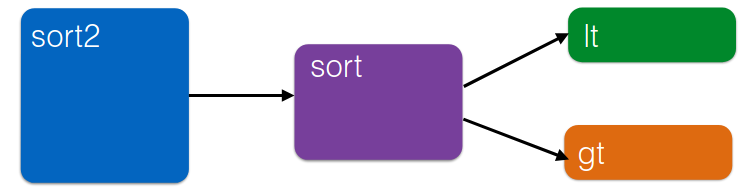
\includegraphics[width=0.8\linewidth]{img/cfi/call1}
\end{center}

Permette di rappresentare il \textbf{flusso di chiamate} all'interno del control flow, ma si tratta di un modello piuttosto permissivo: rappresenta le chiamate ma non il flusso reale delle funzioni. 

Idealmente vorremmo un modello più restrittivo, ovvero il CFG; si introducono i \textbf{basic blocks}: dei contenitori di istruzioni sequenziali terminate da un'istruzione di salto, di qualsiasi tipo (\texttt{jmp}, \texttt{ret}, \texttt{\dots}). Permette di distinguere \texttt{call} dai \texttt{return}, il grafo sul codice di prima diventa:
\begin{center}
	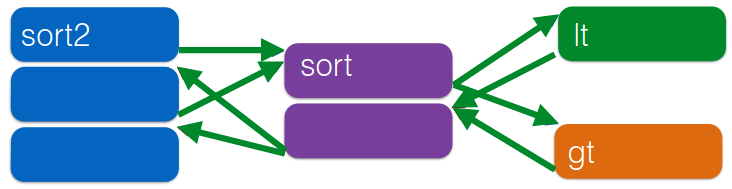
\includegraphics[width=0.8\linewidth]{img/cfi/call2}
\end{center}

Ogni funzione viene "spezzata" in moduli, ognuna delle quali ha una call/return, definendo meglio il modello di esecuzione del programma. Ogni basic block fa una call o una return (praticamente un gadget). 

In sostanza: 
\begin{itemize}
	\item viene calcolato il CFG di call/return a compile time (o comunque partendo dal binario)
	\item il control flow del programma viene monitorato dall'interno, assicurando che segua percorsi definiti dal CFG
	\item le direct calls non vanno monitorate (assumendo che il codice sia immutabile, l'indirizzo target non può essere cambiato), quindi \textbf{solo le indirect calls vanno controllate} (\texttt{jmp}, \texttt{call}, \texttt{ret} con target non costanti, tutti i salti parametrici)
\end{itemize}

\subsection{In-Line Monitor}

Bisogna implementare all'interno del programma un metodo efficace per controllare "da dove arriva" un salto, inoltre deve essere una "trasformazione" del programma. Per fare ciò vengono usate delle \textbf{label}:
\begin{itemize}
	\item viene inserita una label all'inizio del basic block destinazione del salto, come commento, riga non di codice
	\item prima di saltare, viene fatta una \texttt{cmp} tra il valore presente nella destinazione (dove punta il registro su cui viene fatto il salto) e il valore che dovrebbe avere la label
	\item se coincidono tutto a posto, manda avanti l'esecuzione
	\item se non coincidono blocca il programma
\end{itemize} 

Il codice
\begin{table}[h]
	\centering
	\begin{adjustbox}{max width=\textwidth}
	\begin{tabular}{@{} lll | lll @{}}
		\multicolumn{3}{c}{\bfseries Source} & \multicolumn{3}{c}{\bfseries Destination} \\
		\cmidrule(lr){1-3} \cmidrule(l){4-6}
		\bfseries Opcode bytes & \bfseries Instructions &
		& \bfseries Opcode bytes & \bfseries Instructions & \\
		\midrule
		\texttt{FF E1} & \texttt{jmp ecx} & \texttt{; computed jump}
		& \texttt{8B 44 24 04} & \texttt{mov eax, [esp+4]} & \texttt{; dst} \\
		\multicolumn{6}{c}{\dots} \\
	\end{tabular}
	\end{adjustbox}
\end{table}

Diventa:

%--- Instrumented Instructions Table
\begin{table}[h]
	\centering
	\begin{adjustbox}{max width=\textwidth}
	\begin{tabular}{@{} lll | lll @{}}
		\multicolumn{3}{c}{\bfseries Source} & \multicolumn{3}{c}{\bfseries Destination} \\
		\cmidrule(lr){1-3} \cmidrule(l){4-6}
		\bfseries Opcode bytes & \bfseries Instructions &
		& \bfseries Opcode bytes & \bfseries Instructions &\\
		\midrule
		\texttt{81 39 78 56 34 12}
		& \texttt{cmp [ecx],\,12345678h} & \texttt{; comp ID \& dst}
		& \texttt{78 56 34 12} & \texttt{data 12345678h} & \texttt{; ID} \\
		\texttt{75 13}
		& \texttt{jne \_error\_label} & \texttt{; if \(\neq\) fail}
		& \texttt{8B 44 24 04} & \texttt{mov eax, [esp+4]} & \texttt{; dst} \\
		\texttt{8D 49 04}
		& \texttt{lea ecx,[ecx+4]} & \texttt{; skip ID at dst}
		& \multicolumn{3}{c}{\dots} \\
		\texttt{FF E1}
		& \texttt{jmp ecx} & \texttt{; jump to dst}
		& & & \\
	\end{tabular}
	\end{adjustbox}
\end{table}

Viene inserita una label per ogni basic block, quando c'è un indirect call il programma controlla che la destinazione abbia la label corretta (o una delle label corrette) prima di saltare. Controlla che il salto sia alla destinazione corretta.

\paragraph{Tipi di labeling:} Il \textbf{labeling} può essere: 
\begin{itemize}
	\item \textbf{semplice}: una stessa label per tutti i blocchi; evita chiamate fuori dal grafo ma non impedisce salti errati; permette "quello che vuoi" all'interno del grafo
	\item \textbf{dettagliato}: una label diversa a seconda dei punti di ritorno, permettendo di controllare anche che i salti all'interno del grafo siano corretti
\end{itemize}

\paragraph{Can we defeat CFI?}
\begin{itemize}
	\item Code injection con label corretti: non si può fare perché i dati non sono eseguibili (DEP)
	\item Modificare label nel codice per permettere il control flow desiderato: il codice è immutabile
	\item Modificare lo stack durante il check per controllarne l'esito: l'attaccante non può modificare i registri in cui sono caricati i dati rilevanti al controllo (No time-of-check, time-of-use bug TOCTOU)
\end{itemize} 

\paragraph{Garanzie:} Il CFI garantisce di impedire attacchi che modificano il control flow (ROP, ret2libc, \dots). Ma non 
\begin{itemize}
	\item attacchi che manipolano il control flow seguendo le label (mimicry attacks, soprattutto con labeling semplice)
	\item data leaks: hearthbleed non sarebbe stato bloccato
	\item corruptions: modificare variabili di controllo per portare al flusso di esecuzione desiderato (es: overflow di una variabile "\texttt{authenticated}" su cui viene fatto un controllo)
\end{itemize}
	
	% !TeX spellcheck = it_IT

\section{Vulnerabilities Detection}

Dato un programma, si vuole cercare in modo proattivo se sono presenti vulnerabilità. Esistono molti metodi per cercare vulnerabilità, che possono essere più o meno automatici e possono operare in maniera statica o dinamica.
\begin{center}
	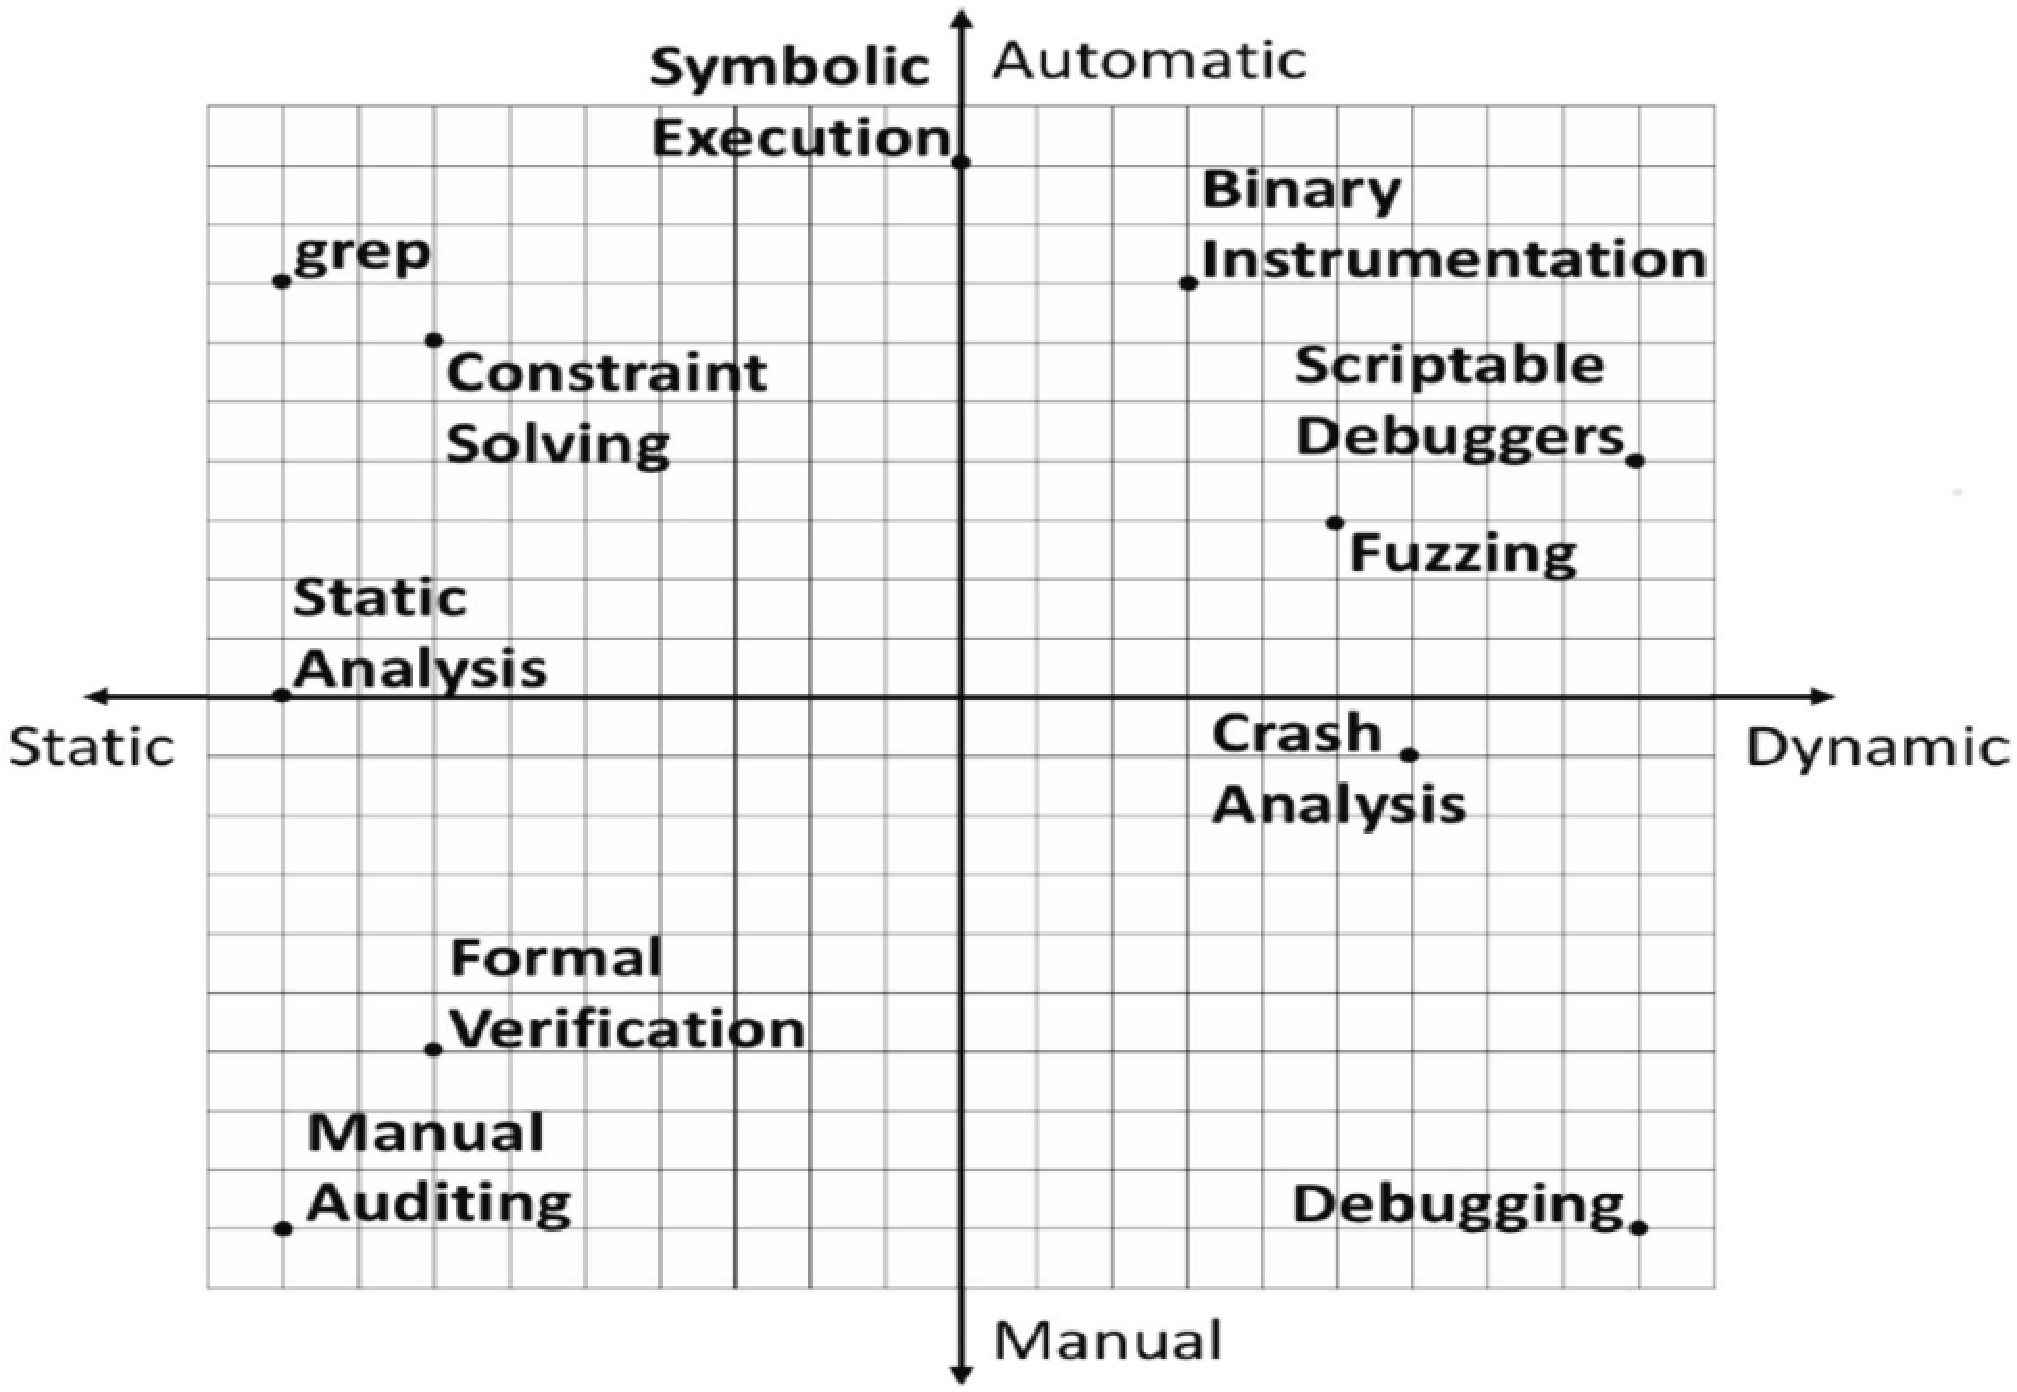
\includegraphics[width=0.6\linewidth]{img/vulnerabilities/manaut}
\end{center}
Di conseguenza, una tecnica può essere
\begin{itemize}
	\item Dinamica e automatica, esempio: binary instrumentation (inserire codice a runtime) o fuzzing (inviare input con l'obiettivo di trovare comportamenti anomali)
	\item Dinamica e manuale, esempio: debugging (eseguire il programma passo-passo per osservarne lo stato interno)
	\item Statica e manuale, esempio: manual auditing del codice (revisione manuale), verifica formale (dimostrare matematicamente la correttezza)
	\item Statica e automatica, esempio: analisi statica, esecuzione simbolica
\end{itemize}

%La symbolic execution nasce come tecnica statica, ma resa dinamica for reasons?\\

%s3?
Prima di effettuare le analisi è necessario definire delle proprietà attribuibili ai tool usati per effettuare le analisi. Le proprietà principalmente sono:
\begin{itemize}
	\item \textbf{Soundness}: una tecnica è \textit{sound} se è in grado di dire che un programma non ha nessuna vulnerabilità, ovvero se c'è una vulnerabilità la trova. Possono esserci \textbf{falsi positivi} (si tratta di un'approssimazione astratta), ma se è presente una vulnerabilità vera la trova. Di conseguenza, un programma è unsound se ci sono dei falsi negativi
	\item \textbf{Completeness}: una tecnica è \textit{complete} se, quando una vulnerabilità viene trovata, questa è vera. Può offrire \textbf{falsi negativi}, ovvero "mancare" vulnerabilità, ma se la trova è sicuramente una vulnerabilità reale. Di conseguenza, una tecnica incomplete può avere falsi positivi
\end{itemize}

\paragraph{TL;DR:} Le tecniche possono essere \textbf{sound}: trova tutti i bug possibili, potrebbe essere un falso positivo, oppure \textbf{complete}: può non trovare tutti i bug, ma se lo trova è una vulnerabilità reale. Ovviamente non esiste un tool che le ha entrambe.\\

Da queste proprietà si possono derivare altre caratteristiche, ad esempio:
\begin{itemize}
	\item se un tool è sound allora vuol dire che considera tutti i path di esecuzione possibili del programma, in quanto requisito per trovare tutti i bug possibili; in maniera dinamica questo non è fattibile, viene fatto tramite tecniche di static analysis, costruendo un'astrazione dell'esecuzione del programma
	\item se un tool è complete allora deve mostrare esecuzioni del programma che permettono di verificare le vulnerabilità; quindi l'analisi è più dinamica, il programma viene lanciato con un set di input che possono causare problemi; la tecnica fornisce input concreti che triggerano vulnerabilità
\end{itemize}
La soundness è più legata alla static analys, mentre la completeness alla dynamic analysis.\\

La \textbf{static analysis} consiste generalmente di modelli matematici astratti per l'esecuzione del programma per poi fare inferenza su quali possibili path potrebbero portare a vulnerabilità. La \textbf{dynamic analysis} invece utilizza esecuzioni più concrete per mostrare vulnerabilità effettive. Solitamente, i tool di detection hanno un approccio ibrido, usando tecniche statiche e dinamiche per ottenere un buon compromesso tra soundness e completeness. Il trade off si traduce in quanti falsi positivi e falsi negativi saranno presenti.\\

Una differenza importante tra static e dynamic execution sono le performance: la static analysis è una analisi del codice, di conseguenza è molto più veloce dell'esecuzione vera e propria del programma (la dynamic deve eseguire davvero il programma, quindi può essere molto lenta). \\

\subsection{Symbolic Execution}

La static analysis è una analisi off-line a partire da codice sorgente o binario del programma, quindi produce risultati riguardo la qualità del codice. Vengono definite delle proprietà a priori sul codice e i tool di static analysis controllano che queste vengano rispettate. \\

Un classico esempio di analisi statica è il compilatore di un programma: per la compilazione e ottimizzazione bisogna effettuare un'analisi del codice; molti tool di analisi statica si basano su ciò che produce il compilatore. L'analisi statica può usare o meno l'esecuzione simbolica.\\

La symbolic execution è una tecnica di static analysis che permette di eseguire in maniera off-line un'esecuzione del programma, "finge" un'esecuzione del programma. Si chiama "simbolica" perché vengono usati valori simbolici, viene calcolata un'approssimazione del programma per ottenere formule che rappresentano lo stato del programma in diversi punti di esecuzione. \\

%cambio slide
Il testing funziona: i bug riportati sono reali, ma ogni test è sostanzialmente un'asserzione, ogni condizione di test può controllare solo una possibile esecuzione. In breve, complete but not sound. Si spera che il caso di test generalizzi abbastanza, ma non ci sono garanzie.\\

La symbolic execution generalizza quello che è il testing di casi singoli, vuole essere "più sound", rappresentando più in generale l'esecuzione del programma. Da asserzioni su input concreti passa ad asserzioni su simboli generici, esempio: 
\begin{center}
	\texttt{assert(f(3) == 5)} $\longrightarrow$ \texttt{y = a; assert(f(y) == 2*y-1);}
\end{center}

Se il path di esecuzione dipende da variabili sconosciute, l'esecuzione simbolica viene divisa concettualmente
\begin{center}
	\texttt{int f(int x) { if (x > 0) then return 2*x - 1; else return 10; }}
\end{center}
Una "esecuzione simbolica parallela".\\

Esempio: 
\begin{center}
	\begin{minipage}{0.78\linewidth}
		\begin{minted}{c}
int a = alpha, b = beta, c = gamma; // symbolic!
int x = 0, y = 0, z = 0;
if (a) {
	x = -2;
}
if (b < 5) {
	if (!a && c) { y = 1; }
	z = 2;
}
assert(x+y+z != 3)
		\end{minted}
	\end{minipage}
\end{center}

\begin{center}
		\begin{tikzpicture}[
	level 1/.style={sibling distance=100mm},
	level 2/.style={sibling distance=70mm},
	level 3/.style={sibling distance=35mm},
	level 4/.style={sibling distance=22mm},
	]
	\node {$x=0, y=0, z=0$}
	child {
		node {$\alpha$}
		child { 
			node {$x=-2$}
			child {
				node {$\beta < 5$}
				child {
					node {$z = 2$}
					child {
						node {\color{g}$\alpha \wedge (\beta < 5)$}
					}
					edge from parent 
					node[left] {$t$}
				}
				child {
					node {\color{g}$\alpha \wedge (\beta \geq 5)$}
					edge from parent 
					node[right] {$f$}
				}
			}
			edge from parent 
			node[left] {$t$}
		}
		child {
			node {$\beta < 5$}
			child{
				node {$\neg \alpha \wedge \gamma$}
				child{
					node {$y=1$}
					child {
						node {$z=2$}
						child {
							node {\color{red} $\neg \alpha (\beta < 5) \wedge \gamma$}
						}
					}
					edge from parent 
					node[left] {$t$}
				}
				child {
					node {$z=2$}
					child{
						node {\color{g} $\neg \alpha \wedge (\beta < 5) \wedge \neg \gamma$}
					}
					edge from parent 
					node[right] {$f$}
				}
				edge from parent 
				node[left] {$t$}
			}
			child {
				node {\color{g} $\neg \alpha \wedge (\beta \geq 5)$}
				edge from parent 
				node[right] {$f$}
			}
			edge from parent 
			node[right] {$f$}
		}
	};
\end{tikzpicture}
\end{center}

Non voglio eseguire realmente il programma, ma si vuole verificare che non ci possa mai essere un'esecuzione del programma che viola determinate proprietà. Voglio vedere se esiste una classe di input che permette di violare le condizioni di esecuzione del programma.\\

\newpage

Per ogni terminazione di path di esecuzione sarà presente una \textbf{path condition}: una formula che permette di individuare tutti gli input che permettono di eseguire quel determinato path (nell'esempio: in verde se soddisfacibili, rosse altrimenti); se tutte le condizioni sono verificate (e quindi l'equazione logica è risolta) vuol dire che gli input permettono di entrare in quel determinato path di esecuzione.\\

Ogni foglia dell'albero di esecuzione ha legata la sua equazione logica che permette di stabilire i potenziali input che portano l'esecuzione in quel determinato path.\\

Se trovo una violazione delle asserzioni in un determinato path, risolvendo la path condition ottengo la classe di input che causa la violazione dell'asserzione. Dalla formula si può derivare l'input concreto per la violazione. Trovare input per la violazione diventa problema per un \href{https://en.wikipedia.org/wiki/Constraint_programming}{\texttt{constraint solver}} (come ad esempio \href{https://github.com/z3prover/z3}{\texttt{Z3}}).\\

Ogni path dell'esecuzione simbolica rappresenta più esecuzioni del programma: esattamente il set di esecuzioni i cui valori concreti soddisfano la path condition. In questo modo si possono coprire molte parti di esecuzione e testing.\\

Vista come analisi statica, la symbolic execution è
\begin{itemize}
	\item \textbf{complete}, ma \textbf{non sound} (generalmente non termina, si "incastra" spesso, la terminazione non è garantita)
	\item dipendente da path, flow e contesto
\end{itemize}

L'idea è piuttosto vecchia, ma aveva dei limiti che la rendevano poco pratica, in particolare: può essere molto compute-intensive: i path possibili possono essere \textit{tanti}, con path condition lunghe e difficili da verificare (anche solo la soddisfacibilità); quindi soggetta all'hardware del tempo: ad oggi hardware e algoritmi per i SMT/SAT solver sono molto migliorati.\\
Nel 2005-2006 è stato ripresa l'idea di symbolic execution per l'ambito del bug finding, con l'aggiunta di euristiche per ridurre lo spazio di esecuzione.\\

\newpage

\paragraph{Symbolic variables:} All'interno delle espressioni (quindi all'interno del linguaggio) vengono \textbf{aggiunte variabili simboliche}, le quali rappresentano valori sconosciuti. Vengono introdotte quando sono presenti input forniti al programma (\texttt{mmap}, \texttt{read}, \texttt{write}, \texttt{\dots}). Se un bug viene trovato queste permettono di riprodurlo. Sono dei "placeholder" per valori sconosciuti a compile time (noti solo durante l'esecuzione).\\

Vogliamo fare in modo che il linguaggio possa includere espressioni simboliche. Normalmente, le variabili in un programma contengono valori, ora possono contenere anche espressioni simboliche. \\

Esempio: 
\begin{center}
	\begin{minipage}{0.3\linewidth}
		\begin{minted}{c}
x = read();
y = 5 + x;
z = 7 + y;
a[z] = 1;
		\end{minted}
	\end{minipage}
	\hfill
	\begin{minipage}{0.6\linewidth}
		La memoria simbolica conterrà: 
		\begin{center}
			\begin{tabular}{l l l}
				\texttt{x} & $\mapsto$ & $\alpha$ \\
				\texttt{y} & $\mapsto$ & \texttt{5+$\alpha$} \\
				\texttt{z} & $\mapsto$ & \texttt{12+$\alpha$}
			\end{tabular}
		\end{center}
		E se \texttt{a} non è abbastanza grande, il valore di $\alpha$ potrebbe causare problemi.
	\end{minipage}
\end{center}

Il \textbf{controllo del programma} può essere \textbf{condizionato dai valori simbolici} (il programma dipende anche dai valori esterni, generalmente). Esempio:
\begin{center}
	\begin{minipage}{0.3\linewidth}
		\begin{minted}{c}
x = read();
if (x>5) {
   y = 6;
   if (x<3)
      y = 5;
} 
else 
   y = 0;
		\end{minted}
	\end{minipage}
\end{center}

E possiamo rappresentare l'influenza dei valori simbolici attraverso le path conditions. Esempio: l'esecuzione arriva alla riga \texttt{3} solo se la path condition $\pi = \alpha > 5$, mentre alla riga \texttt{5} si arriva solo se $\pi = \alpha > 5 \wedge \alpha < 10$.\\

%L'esecuzione del programma può essere modificata considerando le path condition. Esempio:
%s15

Una path condition può essere insoddisfacibile: \textbf{unfeasible path} (non c'è soluzione alla formula logica). Le soluzioni a path constraints possono essere usate come input concreti.\\

Si possono introdurre asserzioni che permettono di determinare se ci sono vulnerabilità sfruttando la feasibility dei path. Esempio: prima di accedere ad un array si introducono dei bound check:
\begin{center}
	\begin{minipage}{0.35\linewidth}
		\begin{minted}{c}
x = read();
y = 5 + x;
z = 7 + y;
if(z < 0)
   abort();
if(z >= len(a));
   abort();
a[z] = 1;
		\end{minted}
	\end{minipage}
\end{center}

Le due condizioni permettono di controllare non ci siano buffer overflow all'interno del programma. Trovare delle soluzioni alle path condition rilevanti (nell'esempio, per la riga \texttt{5} $\pi  =12 + \alpha < 0$ e \texttt{7} $\pi = \neg (12 + \alpha < 0) \wedge 12 + \alpha \geq 4$) vuol dire trovare classi di input che permettono di avere la vulnerabilità per cui si sta testando (buffer overflow in questo caso).\\

Ogni volta che si presenta un branch si ha una fork dell'esecuzione simbolica: si ha un symbolic executor per ogni path di esecuzione. Accade quando si possono avere soluzioni sia alla path condition che alla sua negazione. \\

\paragraph{Libraries e codice nativo:} L'esecuzione simbolica prima o poi raggiungerà i "limiti" dell'applicazione: librerie, sistema o chiamate a codice assembly. Le soluzioni a questo problema possono essere: 
\begin{itemize}
	\item far entrare il symbolic executor nella libreria, ma potrebbero essere \textit{molto} complicate (probabilmente si incastrerà)
	\item fornire un modello delle librerie per l'esecuzione
\end{itemize}

\newpage

\subsubsection{Concolic Execution}

Anche chiamata \textbf{dynamic symbolic execution}, il nome viene da concrete+symbolic. Lavora con gli stessi concetti della symbolic execution ma è un ibrido tra analisi statica e dinamica. \\

Si instrumenta il programma per fare symbolic execution durante l'esecuzione: a partire da un input concreto si esegue il programma, ma si traccia l'esecuzione simbolica durante l'esecuzione concreta; si tiene traccia delle path condition (shadow memory). Ogni volta che si trova un ramo condizionale nel flusso di controllo si tiene traccia del ramo percorso concretamente e la condizione per percorrerlo.\\

Terminata l'esecuzione di un percorso, si ottiene una path condition "completa", per generare un percorso alternativo da eseguire si nega una delle condizioni e si usa un constraint solver per trovare un nuovo input che soddisfa tali condizioni.\\

Si esplora un percorso alla volta tramite valori concreti. Permette di avere sempre dei valori concreti per ogni esecuzione e si possono anche seguire chiamate esterne al programma (perdendo symbolic-ness). Si possono gestire casi senza necessariamente far esplodere la complessità per il SMT solver.\\

% End L9

%L11 Here

% Continuo Symbolic Execution
In breve, la concolic execution parte da input simbolici concreti, alle variabili simboliche si associa un valore concreto in modo da ottenere un'esplorazione del programma secondo il valore scelto. Per ogni diramazione del programma viene salvato lo stato che ha portato ad una determinata scelta all'interno di una shadow memory; vengono salvate tutte le condizioni che vengono attraversate. Una volta arrivato alla fine del path (di una esecuzione) si può tornare indietro per determinare una condizione che permette di esplorare il path simmetrico (un altro path).\\

\newpage

\subsubsection{Search}

Le principali problematiche legate all'utilizzo della symbolic execution sono:
\begin{itemize}
	\item come effettuare l'esplorazione all'interno del flusso di esecuzione di un programma?
	\item risolvere molte formule logiche, anche di grande dimensione, quindi serve un SMT solver e sono rilevanti le performance
\end{itemize}

\paragraph{Path Explosion:} Solitamente la symbolic execution \textit{non può essere svolta in modo esaustivo}, il numero di esecuzioni è (solitamente) esponenziale nel numero di branch (ad esempio, per ogni \texttt{if} di controllo, se ci sono 3 variabili simboliche booleane si possono avere $2^3$ path possibili; ma anche per ogni loop, in quanto possono essere visti come una serie di condizioni).\\

Comparandola all'\textbf{analisi statica}: quest'ultima permette di approssimare \textit{sempre} l'esecuzione di un programma, loop e condizioni possono essere approssimati come "always feasible"; questo semplifica l'analisi ma può portare a \textbf{falsi positivi}. \\

Questo non è vero nella symbolic execution: va \textbf{sempre simulata l'esecuzione di un programma}, con la relativa risoluzione di formule logiche.\\

Bisogna \textbf{definire} dei \textbf{metodi di esplorazione} del path di esecuzione in modo da \textbf{guidare l'esploratore simbolico}, in quanto non è possibile eseguire il programma esaustivamente, bisogna aggiungere delle euristiche per capire \textit{dove andare}. \\

L'idea più semplice possibile è una BFS/DFS, con la relativa queue/stack per tenere traccia di cosa visitare; visito un grafo in maniera "banale". Questo però ha dei problemi: 
\begin{itemize}
	\item il principale è che non sono guidati da nessun tipo di informazione aggiuntiva, non viene cercato nulla di "particolare" all'interno del programma
	\item la DFS potrebbe "bloccarsi in una zona del programma"
	\item la BFS è marginalmente meglio, ma non è facilmente implementabile come concolic
\end{itemize}

\paragraph{Search strategies:} Dobbiamo fornire delle priorità per la ricerca, vogliamo andare verso path che \textit{probabilmente} contengono errori. Vogliamo modellare l'esecuzione del programma come un DAG (Directed Acyclic Graph) in cui i nodi sono gli stati del programma e gli archi indicano la possibile transizione da uno stato all'altro. Di conseguenza dobbiamo decidere \textit{che tipo di algoritmo per l'esplorazione del grafo}.\\

Non è noto \textit{a priori} che path vanno presi, quindi una certa quantità di randomness può essere utile. Alcune idee:
\begin{itemize}
	\item scegliere il path da esplorare in modo uniformemente casuale
	\item random restart se la ricerca non ha trovato nulla di interessante \textit{da un po'}
	\item scegliere casualmente da path con la stessa priorità
\end{itemize}

Uno dei problemi con la randomness è la riproducibilità: vanno \textbf{mantenuti i valori dell'esecuzione}, altrimenti potrebbe non essere chiaro come un bug si è presentato; la comparsa dell'errore può essere legata ad una certa sequenza di stati precedenti, i.e., non è un singolo input che fa crashare il programma ma una sequenza; nel concreto vuol dire \textbf{tenere traccia dei path percorsi}, generalmente tramite il seed di  un generatore pseudo-random.\\

\paragraph{Coverage-guided heuristic:} Tecnica di ricerca basata sul numero di volte in cui viene visitata una determinata istruzione. Il programma è composto da un determinato numero di istruzioni, aggiungo uno "score" per indicare quante volte è stata eseguita ogni istruzione. L'idea è che gli errori sono spesso in aree del programma difficili da raggiungere, quindi si punta a coprire la maggiore percentuale del programma possibile. Quando il punteggio è troppo alto si cercano input per zone ancora non esplorate.\\

Per arrivare in una certa zona di memoria potrebbero servire determinate precondizioni, non sempre soddisfacibili, non è detto che l'esecuzione riesca sempre a visitare tutte le zone del programma.\\

\paragraph{Generational search:} Ibrido tra BFS e coverage-guided
\begin{itemize}
	\item la prima generazione comincia con una esecuzione random completa
	\item tutte quelle successive negano un branch dell'esecuzione ottenuta nella generazione precedente in modo da ottenere un nuovo percorso, con path prefix divers 
\end{itemize}
Vengono usate coverage heuristics per determinare delle priorità.\\

\paragraph{Combined search:} Effettuare più ricerche allo stesso tempo, non esiste una soluzione one-size-fits-all, quindi potrebbe essere un'idea usare algoritmi di ricerca diversi (magari in maniera alternata) per raggiungere parti diverse del programma, sperando di avere una ricerca il più completa possibile.\\

\subsubsection{SMT Solvers}

Per esplorare nuovi path serve risolvere formule logiche, anche molto complesse, quindi le \textbf{performance degli SMT solver} sono fondamentali per effettuare symbolic execution.\\

Da una parte si cerca di \textbf{semplificare le formule} (ad esempio con la concolic execution, inserire input concreti riduce le variabili della formula logica), ma dall'altro si cercano \textbf{ottimizzazioni per la risoluzione delle formule stesse}: i constraint solver usano tecniche per migliorare le performance come: tradurre strutture di memoria in formule logiche efficientemente, teoria degli array (mappare array a formule logiche), caching di richieste precedenti, rimuovere variabili ridondanti, \dots.\\

Alcuni SMT solver:
\begin{itemize}
	\item \href{http://z3.codeplex.com/}{\texttt{Z3, da Microsoft research}}
	\item \href{http://yices.csl.sri.com/}{\texttt{Yices, da SRI}}
	\item \href{https://sites.google.com/site/stpfastprover/}{\texttt{STP, da Vijay Ganesh, now @ Waterloo}}
	\item \href{http://www.cs.nyu.edu/acsys/cvc3/}{\texttt{CVC3, primariamente da NYU}}
\end{itemize}

\newpage

\subsubsection{Symbolic Execution Systems}

Dopo l'ideazione il primo revival della symbolic execution arriva con due sistemi:
\begin{itemize}
	\item \href{https://web.eecs.umich.edu/~weimerw/590/reading/p213-godefroid.pdf}{\texttt{DART: Godefroid and Sen, PLDI, 2005}}
	\item \href{https://www.cs.umd.edu/class/fall2023/cmsc614/papers/exe.pdf}{\texttt{EXE: Cadar, Ganesh, Pawlowski, Dill, and Engler, CCS 2006}}
\end{itemize}

\paragraph{SAGE:} Concolic executor sviluppato da Microsoft Research, nato dal lavoro su DART, usa generational search e viene usato principalmente per trovare bug all'interno di file parser (probabilmente terminano, il comportamento è solo input/output, la concolic execution funziona bene). \\

Viene usato in produzione da MS dal 2007, rappresenta il laboratorio di fuzzing più grande al mondo (più di 500 machine years), con più di 3.4 miliardi di constraint controllati (più grande uso di SMT solver di sempre) per trovare centinaia di bug in centinaia di applicazioni.\\

\paragraph{KLEE:} Esegue simbolicamente bytecode LLVM (compila file a \texttt{.bc}, KLEE lavora su questi). Sviluppato a partire da EXE, lavora usando diverse strategie di ricerca, principalmente random path + converage guided. Simula l'ambiente per gestire system calls, accessi ai file, etc. Disponibile assieme a LLVM.\\

\paragraph{Mayhem:} Sviluppato da CMU (Brumley et al), lavora su binari. Usa una ricerca BFS-style assieme a native execution; combina symbolic e concolic. Genera automaticamente report quando trova bug.\\

\paragraph{Mergepoint:} Estende Mayhem con una tecnica chiamata \textit{veritesting}, combina symbolic execution con analisi statiac del codice:
\begin{itemize}
	\item l'analisi statica viene usata per blocchi di codice completi
	\item la symbolic execution per zone più difficili da analizzare (e.g., con loop indefiniti, aritmetica dei puntatori, syscall)
\end{itemize}
Permette un miglior bilanciamento tra solver ed executor, risparmiando tempo e trovando bug più velocemente (copre più del programma nello stesso tempo). Usato per 11,687 bug in 4,379 applicazioni su distribuzione Linux (inclusi nuovi bug in codice altamente testato).\\

\paragraph{Altri:} Alcuni altri esecutori simbolici: 
\begin{itemize}
	\item \textbf{Cloud9}: Parallel, multi-threaded symbolic execution; Extends KLEE (available)
	\item \textbf{jCUTE, Java PathFinder}: symbolic execution for Java (available)
	\item \textbf{Bitblaze}: Binary analysis framework (available)
	\item \textbf{Otter}: directed symbolic execution for C (available); give the tool a line number, and it try to generate a test case to get there
	\item \textbf{Pex}: symbolic execution for .NET
\end{itemize}

\paragraph{Alla fine:} La symbolic execution generalizza il semplice testing ed è usato i production code per mote applicazioni (SAGE per Microsoft, Mergepoint per Linux), ed esistono molti tool disponibili liberamente.\\

	% !TeX spellcheck = it_IT
\section{Fuzz Testing}

Il \textbf{fuzzing} rientra tra le tecniche di ricerca di vulnerabilità. Nella sua forma più semplice consiste nell'inviare un'elevata quantità di input automaticamente generati a un target (programma o meno, qualsiasi cosa si debba testare). 

L'obiettivo della ricerca è \textbf{trovare stati invalidi} del programma. Per esempio, su un binario, il fuzzing genera input fino a far crashare il programma.

Ci sono diverse \textbf{tipologie di fuzzer}, si possono categorizzare per due elementi fondamentali: 
\begin{itemize}
	\item il metodo di generazione dell'input
    
	\item introspection: livello di conoscenza del programma
\end{itemize}

\paragraph{Introspection:} Si possono avere 3 livelli principali: 
\begin{itemize}
	\item \textbf{black box}: non sanno nulla di come è formato il programma all'interno
	
    \item \textbf{white box}: conoscenza completa del programma, visione totale dello stato interno del programma
	
    \item \textbf{grey box}: non hanno una visione completa dello stato, ma possono estrarre informazioni a runtime tramite instrumentazione
\end{itemize}

\paragraph{Metodo di generazione input:} Esistono fuzzer che hanno una generazione dell'input di tipo: 
\begin{itemize}
	\item \textbf{generazionale}: partono da zero, generano secondo una grammatica, espressioni regolari o regole più complesse (online learning, ML)
	
    \item \textbf{mutazionali}: viene fornito un set di input di partenza, a ogni iterazione il fuzzer muta il set di input alla ricerca di altri input "\textit{interessanti}" (va definito cosa significa)
	
    \item \textbf{ibrido}: combina tecniche di generazione e mutazione
\end{itemize}

\subsection{Fuzzer Architecture}

\textit{Come è fatto un fuzzer?} Nella forma più semplice si hanno da un lato il fuzzer, il programma dall'altro: vengono mandati input da una parte all'altra.

\paragraph{LibAFL:} Libreria Rust che permette la creazione di fuzzer arbitrariamente complessi. Per andare un po più nel dettaglio
\begin{center}
	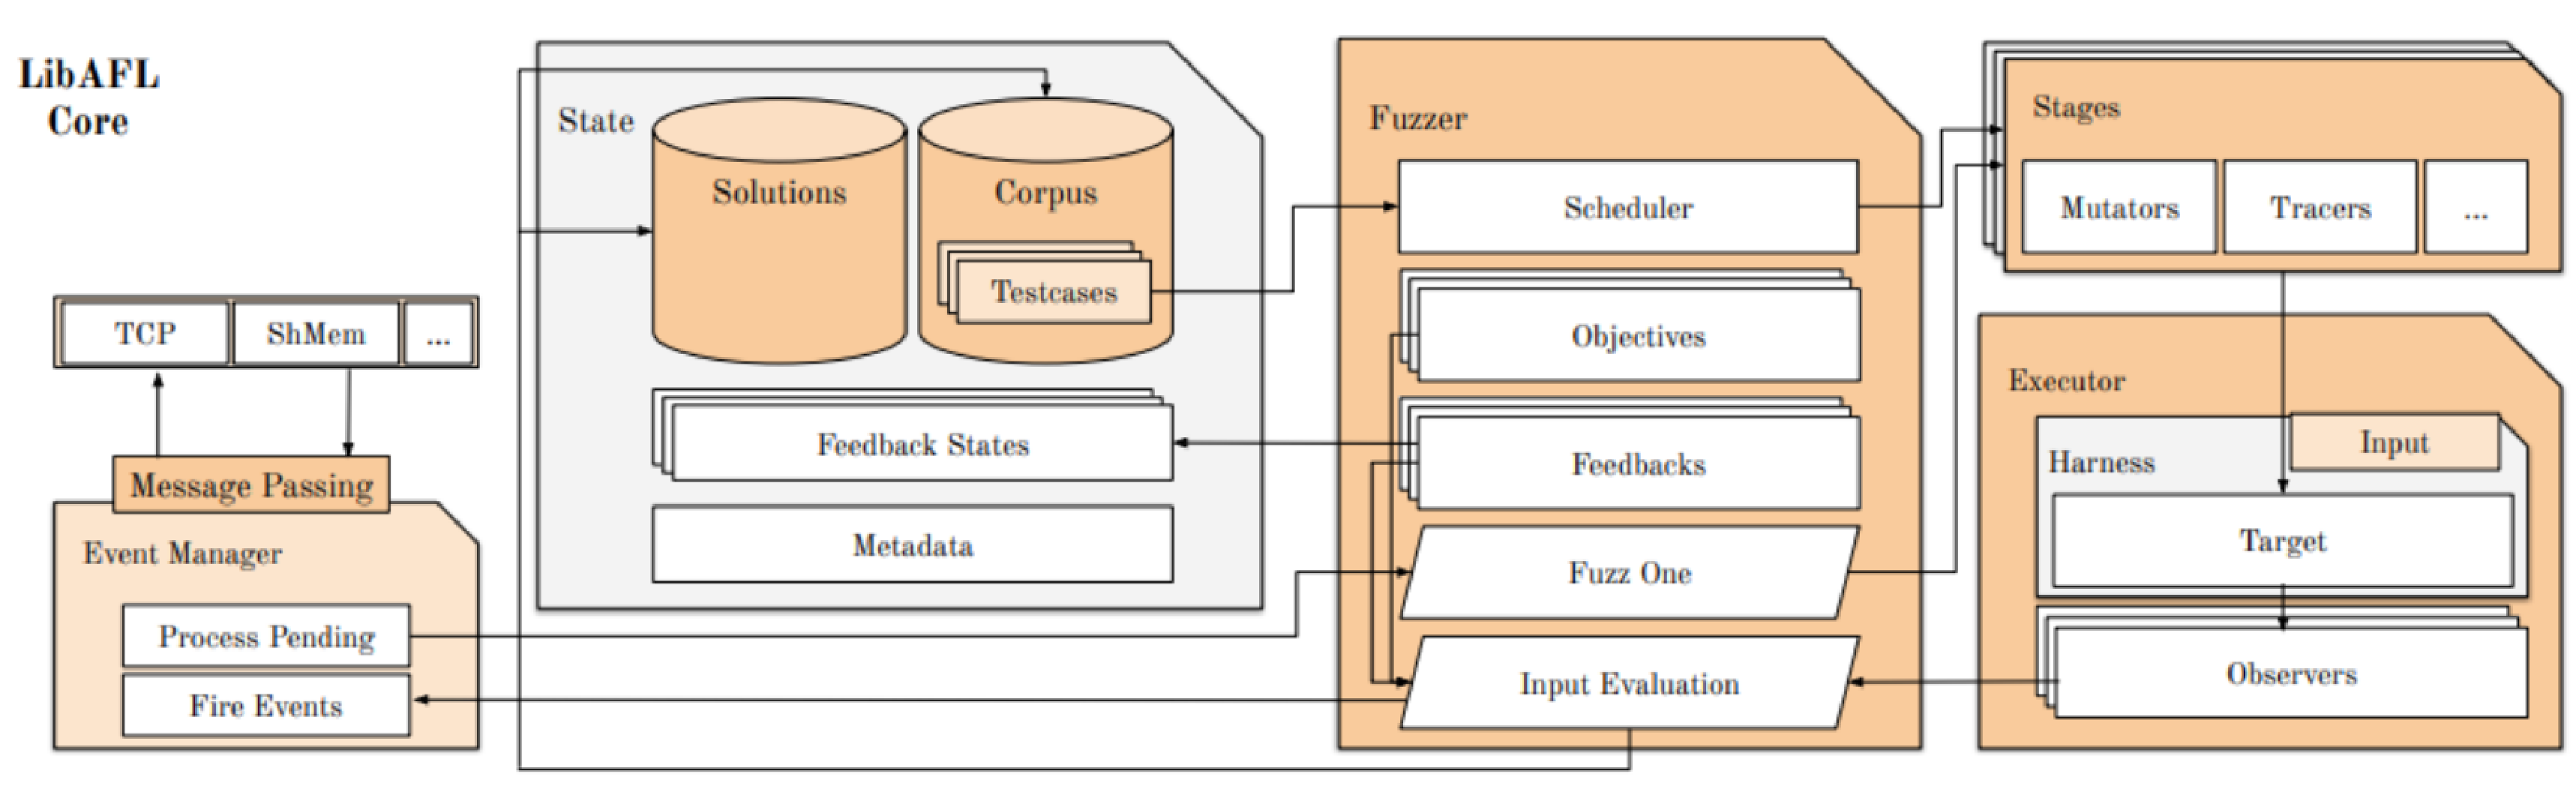
\includegraphics[width=\linewidth]{img/fuzzing/fuzzercore}
\end{center}

\paragraph{Executor:} Si tratta del componente che \textbf{riceve l'input} da parte del fuzzer vero e proprio \textbf{per poi eseguirlo}. Si possono avere diversi livelli di complessità per un executor, il più semplice (per un binario) è un fork server (fork del processo per poi applicare l'input, la fork evita di dover ricaricare il programma in memoria, il che sarebbe troppo lento). 

Altre tipologie di executor, ad esempio per un kernel, dato che non si può caricare un kernel ex novo ad ogni test, usano VM o Hypervisor (wrapper attorno all'executor vero e proprio).

\paragraph{Input:} Rappresentazione astratta della \textbf{tipologia di input accettata} dal programma. Potrebbe essere una bytestring (binario), una sequenza di syscall (kernel), una lista di transazioni (smart contract), \dots; a seconda di ciò che viene testato è importante conoscere cosa prende in input il programma.

\paragraph{Corpus:} Gli input vanno salvati da qualche parte. Il Corpus contiene due elementi:
\begin{itemize}
	\item \textbf{Solutions}: input che assolvono al loro compito; ovvero causano crash o comunque raggiungono l'obiettivo

	\item \textbf{Interesting}: input che raggiungono zone \textit{interessanti} del programma (e quindi vengono messi in coda per eventuale mutazione)
\end{itemize}
Quelle non interessanti vengono scartate (a cosa servono?).

\paragraph{Generator:} Il componente che si occupa di generare input, secondo grammatiche o regole di generazione. In generale, gli input generati devono rispettare una struttura.

\paragraph{Scheduler:} Si può avere un numero indefinito di test case (tra generazione e mutazione gli input possono aumentare molto in fretta), quindi è importante orchestrare in maniera corretta la \textbf{selezione dei test case}. Va definito uno scheduler, nel caso più semplice può essere una coda/stack, ma può avere un impatto significativo sulle performance.

\paragraph{Stage:} Definisce una serie di operazioni da effettuare sull'input (ricevuto dallo scheduler), come mutazioni, taint tracking, \dots.

\paragraph{Mutator:} Si occupa della \textbf{mutazione degli input}. A seconda del test case e di ciò che si vuole ottenere ne esistono di diverso tipo, il metodo più semplice è un bit flip, ma anche splicing, block swapping, truncating, \dots; possono essere usate tecniche arbitrariamente complesse.

\paragraph{Observer:} Si vuole avere conoscenza di ciò che accade all'interno del programma, al fine di definire \textit{cosa è interessante} (tranne nei casi di fuzzer black box, dove non si ha la nozione di interessante, vanno più o meno a caso, le uniche cose interessanti sono le soluzioni). 

L'observer si occupa di \textbf{estrarre} (in qualche modo) \textbf{informazioni dal programma} in fase di analisi per poi rimandarle al fuzzer. 

Un esempio potrebbe essere una coverage map: controlla gli edge, vengono tracciati i possibili flussi di esecuzione e si tiene traccia in un bytearray di quante volte l'esecuzione passa attraverso ogni determinata zona del programma.

\paragraph{Feedback:} Modulo che si occupa di \textbf{analizzare le informazioni estratte}, controparte dell'observer. Riceve l'output dell'observer, lo analizza per determinare caratteristiche riguardo al test case eseguito, ad esempio per stabilire se è interessante e aggiungerlo o meno al corpus.

Cosa manca? Altri componenti che potrebbero esserci, meno nel dettaglio: 
\begin{itemize}
    \item se il fuzzer è su una macchina diversa dall'eseguibile, bisogna collegarlo alla rete
    \item \textbf{Harness}: sotto-componente dell'executor che effettivamente passa l'input al programma
\end{itemize}

\subsubsection{Instrumentation}

\textit{Come si fa a implementare un observer?} Vogliamo estrarre informazioni da un programma a runtime, solitamente si fa con tecniche di \textbf{instrumentazione}: tipicamente a partire da una intermediate representation (per poterlo analizzare più facilmente in maniera automatica, senza rischiare di modificare il comportamento originario del programma), si analizza il programma per identificare zone "interessanti" e si aggiungono istruzioni che permettono di capire quando queste vengono raggiunte. 

Esempio: mi interessa (per qualche motivo) contare le chiamate di sistema del programma, cerco all'interno della intermediate representation tutte le istanze di syscall e assegno un ID ad ognuna di queste, il codice iniettato tramite instrumentazione incrementerà in un array la casella corrispondente alla syscall effettuata, per ogni chiamata all'interno del programma. 

Altro esempio di instrumentazione: i fat pointer, obiettivo diverso, ma sostanzialmente è la stessa cosa (visti qui: \ref{par:fat-pointers}). 

\paragraph{TL;DR:} Instrumentazione vuol dire modificare il binario (solitamente non da sorgente, ma da rappresentazione intermedia), per rilasciare informazioni a runtime.

\subsubsection{Sanitizers}

Vogliamo identificare crash del programma, ma potrebbe non bastare per trovare vulnerabilità. Per questo motivo sono nati i sanitizer, pezzi di codice, \textbf{instrumentazioni aggiuntive} che permettono di \textbf{rilevare comportamenti anomali} quando accadono. 

Esempi: 
\begin{itemize}
	\item \href{https://github.com/google/sanitizers/wiki/addresssanitizer}{\texttt{AddressSanitizer (ASan)}}, rileva errori di memoria

	\item \href{https://docs.kernel.org/dev-tools/ubsan.html}{\texttt{UndefinedBehaviorSanitizer (UBSan)}}, rileva undefined behavior

	\item \href{https://github.com/google/sanitizers/wiki/threadsanitizercppmanual}{\texttt{ThreadSanitizer (TSan)}}, rileva race conditions
\end{itemize}

Quando rilevano un'anomalia fanno crashare il programma, con un log relativo all'errore, il quale può essere più o meno dettagliato.

Esempio: ASan (tra le altre cose) aggiunge delle "red zone" attorno alle zone di memoria, ovvero zone senza permessi di lettura o scrittura: quando il programma prova ad accedervi si genera un \texttt{segfault}. Instrumenta il programma per cercare tutte le allocazioni, tutti gli utilizzi della memoria in generale (con le relative ottimizzazioni, non così semplice).

Ovviamente i sanitizer non vengono usati in produzione, non si tratta di un comportamento desiderato, oltre al fatto che rallentano l'esecuzione.

\vfill

\subsection*{Notes}

\paragraph{State of the Art: AFL++:} Stato dell'arte per fuzzing su binario, \href{https://www.usenix.org/system/files/woot20-paper-fioraldi.pdf}{\texttt{presentato nel 2020}} come gray box fuzzer con edge coverage guidance, derivato dall'originale AFL. Abbastanza customizzabile, scritto in C++. 

\paragraph{NB:} Si può fuzzare un po' tutto, non solo binari. Ad esempio:
\begin{itemize}
	\item \href{https://github.com/google/syzkaller}{\texttt{Syzkaller:}} unsupervised coverage-guided kernel fuzzer

	\item \href{https://softsec.kaist.ac.kr/~sangkilc/papers/choi-ase2021.pdf}{\texttt{Smartian:}} Smart Contract Fuzzing with static and dynamic data-flow analyses

	\item \href{https://dl.acm.org/doi/pdf/10.1145/3492321.3519591}{\texttt{Nyx-Net:}} coverage-guided network testing
\end{itemize}

\paragraph{OSS-Fuzz:} Progetto lanciato da Google nel 2016 per fare fuzzing di repo open source di grossi progetti, individuando un buon numero di vulnerabilità in più di 1000 progetti.

% End L10
	
	% !TeX spellcheck = it_IT
\section{Meltdown and Spectre}

Pubblicati nel 2017, si tratta di attacchi side channel, vanno a distruggere alcune delle assunzioni solitamente fatte sull'hardware. Per quanto riguarda la sicurezza, solitamente vengono fatte assunzioni su alcune proprietà (come ad esempio si presuppone sia presente isolation tra processi, grazie all'MMU), con questi attacchi alcuni componenti hardware non sono più considerabili trusted, \textbf{rompendo il tipico threat model considerato}.

Con questi attacchi è stato mostrato come l'hardware possa essere compromesso, \textit{senza particolari requisiti a livello software} (ovvero funzionano anche con un software bug free). Questi attacchi mostrano come, tramite un processo senza bug non privilegiato, si possa andare a leggere la memoria del kernel. Vengono \textbf{sfruttate problematiche di progettazione hardware} per andare a minare le solite assunzioni sulle componenti fisiche.

Questi attacchi mettono in crisi \textit{tutta la progettazione hardware fino alla loro pubblicazione}, i requisiti di sicurezza non sono mai stati tenuti in considerazione durante la progettazione, sono sempre state guardate prima le caratteristiche funzionali (performance). Non esistono soluzioni ottimali, a meno di ricostruire tutta l'architettura.

Ci sono due principali componenti coinvolti in questi attacchi: 
\begin{itemize}
	\item CPU
    
	\item Cache
\end{itemize}

Le cache possono essere viste come una matrice in cui
\begin{itemize}
	\item le linee si chiamano cache set
	
    \item le colonne si chiamano cache line
\end{itemize}

Tramite una manipolazione dell'indirizzo virtuale si può andare a capire se un determinato dato è presente all'interno della cache (ogni indirizzo virtuale può far riferimento ad una sola linea all'interno della cache). L'indirizzo virtuale (dopo essere stato tradotto in fisico) viene usato per determinare la linea di cache in cui i dati verranno posti. 

Quando un processore deve accedere ad un certo indirizzo, richiede certi dati, prima interroga la cache, solo dopo, se il dato non è stato trovato, viene interrogata la RAM (in seguito ai livelli di cache inferiori).

In generale, in una CPU esistono più tipologie e livelli di cache 
\begin{itemize}
	\item ogni core ha una cache L1 e L2
	
    \item divisa tra i core si ha una cache L3
\end{itemize}
Più le cache sono vicine al core, più sono veloci. Queste tipologie di attacchi lavorano principalmente su cache L3. 

\paragraph{Micro-architecture attack:} Attacchi alla micro-architettura, sono attacchi che si posizionano nel layer tra software e hardware. 

\paragraph{Side channel attacks:} Attacchi (studiati soprattutto in crittografia) che studiano l'ambiente di esecuzione di un processo/dispositivo; anche senza guardare fisicamente all'interno del dispositivo, si possono fare inferenze sul contenuto del dispositivo? Si tratta di inferenze a partire dall'ambiente circostante per dedurre il contenuto.

Esempio: considerando una smart card, l'unica interazione possibile con una smart card è inviare del testo in chiaro e ricevere del testo cifrato (si presuppone che esistano difese hardware contro l'aprire fisicamente la smart card e leggere). Si può guardare l'ambiente esterno alla smart card per capire la chiave, ad esempio, guardando quanta energia elettrica usa la smart card per cifrare il testo: guardando l'onda di esecuzione, ogni testo avrà un'onda differente e si sfrutta conoscenza sull'algoritmo di cifratura per ottenere informazioni sulla chiave usata; ad esempio, alcune ottimizzazioni in base al contenuto di testo e chiave usate dall'algoritmo potrebbero essere indizi. Magari non si può capire la chiave completa, ma capirne il 90\% per poter fare brute force sul resto è good enough.

In generale, l'analisi dell'ambiente circostante ad un dispositivo permette di dedurre informazioni riguardo l'esecuzione.

\subsection{Attacchi alle cache}

Le cache si prestano a questa tipologia di attacchi in quanto condivise, ogni processo condivide la stessa cache. 

Meltdown e Spectre non sono completamente hardware, ma richiedono interazione tra software e hardware (microarchitectural attack).

\subsubsection{Flush \& Reload}

Lo scenario di attacco è: una shared memory (ad esempio, una libreria in comune) e due processi software: un "attaccante" $P1$ e una "vittima" già in esecuzione sulla macchina $P2$. 

Si suppone che $P1$ conosca il codice di $P2$ (ad esempio, implementa un algoritmo noto), ma ovviamente non conosce lo stato di esecuzione del programma (ovvero valori usati all'interno del programma, presenti solo all'interno della memoria del processo $P2$). L'attaccante quindi vuole "spiare" lo stato di esecuzione di $P2$ sfruttando la memoria condivisa, supponendo siano due programmi indipendenti e bug-free.

Il processo $P1$ fa: 
\begin{itemize}
	\item \textbf{flush}: operazione assembly fornita dall'architettura, permette di svuotare totalmente la cache
\end{itemize}

In seguito $P1$ rilascia l'esecuzione e fa andare in esecuzione $P2$, il quale caricherà i suoi valori/eseguirà il suo codice. Una volta eseguito del codice, ogni indirizzo virtuale relativo alle istruzioni eseguite da $P2$ farà riferimento a una linea della cache, i.e., le istruzioni eseguite da quando la cache è stata svuotata saranno state caricate in cache.

Quando $P1$ torna in esecuzione, in seguito a $P2$, farà
\begin{itemize}
	\item \textbf{reload}: carica (accede) ad ogni indirizzo virtuale presente all'interno del codice, per poi calcolare il tempo di accesso a ogni indirizzo (access time)
\end{itemize}

Dal punto di vista della cache, gli unici indirizzi al suo interno sono quelli eseguiti da $P2$:
\begin{itemize}
	\item se un indirizzo non è in cache andrà preso dalla memoria, più lento
    
	\item se il valore è già in cache allora l'accesso sarà molto più veloce
\end{itemize}

Quando viene trovato un tempo di accesso più veloce a una linea di cache, $P1$ può capire quali istruzioni ha eseguito il programma $P2$, ottenendo informazioni anche sullo stato e contenuto della memoria di $P2$. L'unica linea con accesso più veloce è la linea della libreria comune ai due processi già caricata in cache, ovvero le istruzioni appena usate dal secondo processo.

Riassunto: 
\begin{itemize}
	\item $P1$ fa \texttt{flush} della cache
	
    \item $P2$ va in esecuzione, carica in cache delle istruzioni
	
    \item $P1$ tenta di accedere a ogni indirizzo virtuale, quelli con tempo di accesso più breve rispetto agli altri sono le istruzioni eseguite da $P2$
\end{itemize}

Sapendo il mapping di $P2$ e il timing della cache posso inferire lo stato di esecuzione di $P2$.

\subsubsection{Prime \& Probe}

Si hanno lo stesso scenario e assunzioni di prima (so dove come viene mappata virtualmente la memoria di $P2$), ma non si ha una memoria shared in uso da entrambi i programmi.

L'attacco consiste di:
\begin{itemize}
	\item $P1$ fa \textbf{prime} della cache: riempie completamente la cache (semplicemente accedendo a tutti gli indirizzi del suo spazio di indirizzamento che sappiamo essere mappati all'interno di $P2$)
    
	\item va in esecuzione $P2$, eseguirà il suo blocco di codice, caricando $x$ e $y$ in cache
	
    \item $P1$ fa timing sulla cache: prova tutte le linee, quelle eseguite da $P2$ avranno tempo più lento; tutti i dati sono in cache, il codice di $P1$ è diverso da $P2$, quando $P1$ riprova ad accedere a tutta la cache ci saranno delle linee più lente, in quanto richiedono lo scarico e carico della cache: $P2$ avrà usato le linee virtuali corrispondenti a quello slot di cache
\end{itemize}

Ancora una volta, misurando le differenze di timing, si può capire l'indirizzo virtuale utilizzato da un altro processo, sapendo il mapping virtuale di questo secondo processo si può arrivare alle istruzioni eseguite, portando a inferenze sullo stato (utili o meno).

Questi attacchi vengono portati su un unico core, "isolando" l'esecuzione di programma target e attaccante, per evitare che ci sia "noise" a livello di cache dovuto all'esecuzione di altri processi (scheduling).

\subsection{Speculative Execution}

Meltdown e spectre usano vulnerabilità all'interno della CPU. Un'ottimizzazione (abbastanza spinta) della CPU è la \textbf{speculative execution} (presente all'interno di ogni CPU moderna). 

Un programma è costituito di esecuzioni sequenziali: lento. L'esecuzione speculativa è "\textit{tentare di indovinare}" cosa dovrà fare la CPU nei passaggi successivi, vuole parallelizzare il più possibile l'esecuzione delle istruzioni (a livello di micro-operation, più in basso dell'assembly).

Il processore deve capire che istruzioni sono dipendenti tra loro, quali operazioni vanno eseguite in sequenza e quali invece possono essere parallelizzate.

All'interno di una reservation station (shadow memory) la CPU memorizza le istruzioni da eseguire sequenzialmente. 

Ma la "prossima istruzione" che sta tentando di eseguire in anticipo non è detto che andrà effettivamente eseguita (detta transient instruction, sta effettivamente speculando sull'esecuzione); potrebbe succedere qualcosa tra \textit{adesso} e quando dovrà davvero essere eseguita l'istruzione "speculata" che ne evita l'esecuzione (come ad esempio un \texttt{segfault}).

I risultati dell'esecuzione speculativa sono tenuti all'interno di un buffer (ROB), non vengono scritti immediatamente nei registri/memoria dell'architettura finché l'esecuzione non risulta confermata. Tutta la speculazione non è visibile all'architettura finché l'esecuzione non è confermata.
%mdsattacks.com/diagram.html

La domanda che si sono posti meltdown e spectre è: \textit{posso usare questa cosa per fare leak di informazioni?} La risposta è \textit{sì}.

\subsection{Meltdown}

\href{https://meltdownattack.com/meltdown.pdf}{\texttt{Meltdown}} è una vulnerabilità che sfrutta:
\begin{itemize}
	\item speculative execution
	
    \item cache attacks
\end{itemize}

Idea dietro il codice:
\begin{minted}{c}
data = kernel_access[I];
access(probe_array[data*4096]);
address = probe_array + data*4096;
\end{minted}

La prima istruzione è un \textbf{accesso ad un indirizzo del kernel}: siamo in un programma non privilegiato, quindi causerà un \texttt{segmentation fault}. Le istruzioni dopo sono "fattibili" (accessi ad un array definito all'interno del programma), non verranno mai eseguite, il programma si fermerà sempre prima, ma la speculative execution non lo sa e le vede come indipendenti tra loro. 

Ognuna delle operazioni successive verrà divisa in microop ed eseguite in parallelo, il dato non viene faultato subito ma viene eseguito, anche se di nascosto (\textit{se} vince la race condition in cui la seconda istruzione finisce prima della prima all'interno del buffer, ma basta fare qualche tentativo anche nel peggiore dei casi).

Le istruzioni che sono finite in shadow memory vengono \textbf{eseguite e poi bloccate}, l'architettura non le vede, ma finiscono comunque all'interno della \textbf{cache}. Sarà presente all'interno di una linea della cache il valore a cui è stato fatto l'accesso, ma che non doveva essere caricato.

Tramite prime \& probe si può risalire a quale linea kernel (privilegiata) è stato fatto l'accesso. \textit{Ma si può scoprirne il valore?} Per fare ciò entra in gioco la terza istruzione del listato: \texttt{probe\_array} è un valore noto (definito dall'attaccante), \texttt{4096} è la grandezza di una linea della cache (potrebbe essere diversa, esempio di valore) e \texttt{data} è il valore che vogliamo scoprire. In questo modo viene caricata in memoria una cache line diversa in base al valore del dato.

Grazie al timing possiamo capire il valore: l'accesso è più veloce solamente alla linea $x$: il valore di \texttt{data}, caricato durante l'accesso out-of-order era $x$.

\subsection{Spectre}

\href{https://spectreattack.com/spectre.pdf}{\texttt{Spectre}} è una vulnerabilità che sfrutta:
\begin{itemize}
	\item speculative execution
	
    \item cache attacks
	
    \item branch prediction
\end{itemize}

La branch prediction unit è un componente all'interno delle CPU, fa parte (circa) dell'esecuzione speculativa, tenta di prevedere l'esito dei branch per fare speculazione; viene fatto anche in base all'esecuzione passata (e.g., se 99 volte su 100 è entrato nel loop, probabilmente entrerà di nuovo).

Quindi, facendo un accesso a un array, con un indice valido, 99 volte, e alla 100esima viene messo un indice out of bound, la branch prediction eseguirà lo stesso l'istruzione, prima che il programma si accorga che l'accesso non è valido. Il valore caricato dalla branch prediction unit verrà, ancora una volta, caricato in cache.

Similmente a meltdown, un'istruzione che non doveva essere eseguita è stata anticipata, con effetto sulla cache, quindi ne si può capire il valore. 

%End L12 
%Fine corso :-(

\end{document}
